\documentclass[english]{uzhpub}
\usepackage[T1]{fontenc}
\usepackage[latin9]{inputenc}

\usepackage[separate-uncertainty]{siunitx}
\sisetup{
    range-units = single,       % \SIrange soll die Einheit nur einmal anzeigen
    list-units  = repeat,       % \SIlist soll die Einheit wiederholen
}


%% erlaubt Listen einfacher zu formatieren (bietet nosep für kompakte Listen)
\usepackage{enumitem}
%% erlaubt hübsche Tabellen über mehrere Seiten, beinhaltet booktabs (\toprule, \midrule, ...)
\usepackage{ctable}
%% ermöglicht farbigen Text ({\color{red} ...})
\usepackage{xcolor}

%% erweiterte Funktionalität für Formeln (Pakete der American Mathematical Society)
\usepackage{amsfonts,amsmath,amsthm,amssymb}

\usepackage{pdfpages}

\usepackage{graphicx}
%% ermöglicht Bilder und Tabellen am eingegebenen Ort zu platzieren ([H])
\usepackage{float}
%% ermöglicht Unter-Bilder in einer figure-Umgebung
\usepackage{subfig}
%% Grafik-Dateien werden in den folgenden Or\usepackage{braket}dnern gesucht
\graphicspath{{img/}}
%% Grafikdateien haben die folgenden Endungen (höchste Priorität zu erst)
\DeclareGraphicsExtensions{.pdf,.png,.jpg}

%% Vertikaler Abstand zwischen Absätzen, Beginn eines Absatzes nicht einrücken
\usepackage{parskip}
% \setlength{\parskip}{0.6em}   % Vertikaler Abstand zwischen Absätzen anpassen
% \setlength{\parindent}{0em}   % Einrück-Abstand anpassen

%% zeige Labels im Seitenrand. Dies ist praktisch um Verweise zu kontrollieren
\usepackage[final]{showkeys} % die Option 'final' deaktiviert die Ausgabe von showkeys


%% Ermöglicht Links im PDF
%%   sollte möglichst spät in der Präambel geladen werden
\usepackage[
 pdftex,                        % wir verwenden pdftex/pdflatex
 bookmarks=true,                % wir wollen auch im PDF-Reader ein Inhaltsverzeichnis
 bookmarksdepth=3,              % das Inhaltsverzeichnis soll 3 Tiefen enthalten
 colorlinks=true,               % Linktexte sollen Farbig sein
 linkcolor=black,               % Links innerhalb des Dokuments bleiben schwarz
 citecolor=black,               % Links zu Quellenangaben bleiben ebenfalls schwarz
 urlcolor=blue,                 % URL-Linktexte sollen blau dargestellt werden
%  pdfborder={0 0 0}              % Links im PDF erhalten keinen Rahmen, nur nötig wenn colorlinks=false
]{hyperref}

\usepackage{braket}
\usepackage{amssymb}


\begin{document}

%% Titelei
\title{Masterthesis: analysis of $B$ $\rightarrow$ $K^{*}$ $\mu$ $\mu$ decay}

\subtitle{Supervisors: Prof. Dr. Nicola Serra, Dr. Marcin Chzsaszcz}

\author{Author: Oliver Dahme}

%\date{Date}

\maketitle



%% Addpart entspricht dem "Kapiteltitel"
%\addpart{Abstract}

\begin{abstract}
 Here comes the abstract
\end{abstract}

%\addpart{Introduction}

\section{$B$ $\rightarrow$ $K^{*}$ $\mu$ $\mu$ decay}

% The $B$ $\rightarrow$ $K^{*}$ $\mu$ $\mu$ decay has a quark $b \rightarrow s$ transition which is relevant


\subsection{Kinematics}
The Decay is a flavor changing neutral current (FCNC) with four charged particles in the final state: \\
The $K^+$ and $\pi^-$ from the $K^{*}$ decay and two leptons from the loop or box digrams:
\begin{figure}[H]
 \centering
 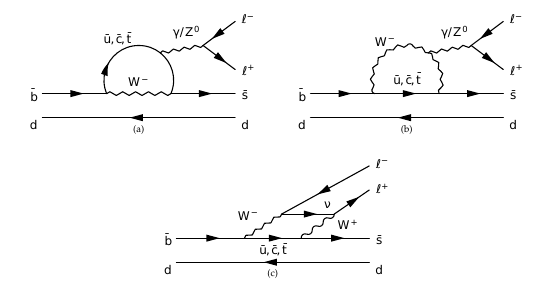
\includegraphics[width=0.8\linewidth]{KstarFeynman}
 \caption{Feynman diagrams for decay $B_d$ $\rightarrow$ $\mu^+$ $\mu^-$ at lowest order}
 \label{fig:Feynman}
\end{figure}
The kinematics of the decay are defined by the three angels $\theta_K$, $\theta_L$ and $\phi$, shown in figure \ref{fig:angels} and the invariant di-muon mass square $q^2$.
\begin{figure}[H]
 \centering
 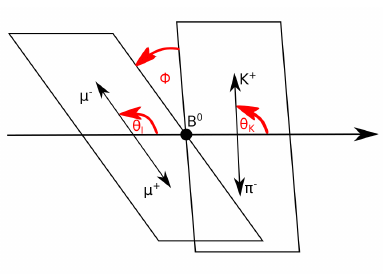
\includegraphics[width=0.6\linewidth]{angels}
 \caption{kinematic variables of the decay $B^0$ $\rightarrow$ $K^{*0}$ $\mu$ $\mu$}
 \label{fig:angels}
\end{figure}
From them one can obatain the differential decay rate for the $B^0$ Meson:
\begin{equation}
 \begin{split}
  \frac{d^4 \Gamma}{d \cos{ \theta_L} d \cos{\theta_K} d \phi d q^2} &= \frac{9}{32 \pi} I(q^2,\theta_L, \theta_K, \phi) \\
  \text{with: } I(q^2,\theta_L, \theta_K, \phi) &= I_1^S \sin{^2(\theta_K)} + I_1^C \cos{^2 \theta_K} + \left(I_2^S \sin{^2 \theta_K} + I_2^C \cos{^2 \theta_K} \right) \cos{^2\theta_L} \\
  &+ I_3 \sin{^2 \theta_K} \sin{^2 \theta_L} \cos{2\phi} + I_4 \sin{2\theta_K} \sin{2\theta_L} \cos{\phi} \\
  &+ I_5 \sin{2\theta_K} \sin{ \theta_L} \cos{ \phi} \\
  &+ \left(I_6^S \sin{^2 \theta_K} + I_6^C \cos{^2 \theta_K}  \right) \cos{ \theta_L} + I_7 \sin{ 2\theta_K} \sin{\theta_L} \sin{\phi} \\
  &+ I_8 \sin{ 2\theta_K} \sin{ 2\theta_L} \sin{ \phi} + I_9 \sin{^2 \theta_K} \sin{^2 \theta_L} \sin{2 \phi}\\
 \end{split}
 \label{eq:diff_decay_rate}
\end{equation}

\subsection{Operators for $B \rightarrow X_s l^+l^-$ decays}
The effective Lagrangian for $B \rightarrow X_s l^+l^-$ decays has the form: \\
\begin{align}
 \mathcal{L}_{eff} & = \mathcal{L}_{QCD,QED}(u,d,s,c,b,e,\mu,\tau) \notag                                                                                           \\
                   & + \frac{4G_F}{\sqrt(2)} \left[ V_{us}^* V_{ub} (C_1^c P_1^u + C_2^c P_2^u) + V_{cs}^* V_{cb} (C_1^c P_1^c + C_2^c P_2^c) \right] \label{eq:La} \\
                   & + \frac{4G_F}{\sqrt(2)} \sum_{i=3}^{10} \left[ (V_{us}^* V_{ub} + V_{cs}^* V_{cb})C_i^c + V_{ts}^* V_{tb} C_i^t  \right]P_i . \notag
\end{align}
The first term in equation \ref{eq:La} contains the kintec terms of the light SM particles as well as their QCD and QED interactions. The remaining two terms consist of $\Delta B = - \Delta S =1$ local operators of dimension $(d \leq 6)$, which contain those light fields. The mass of the s quark can be negleted in comparisson with the b mass. One gets the following operators:
\begin{equation}
 \begin{split}
  \mathcal{O}_1^u &= (\bar{s}_L \gamma_\mu T^a u_L)(\bar{u}_L \gamma^\mu T^a b_L),  \\
  \mathcal{O}_2^u &= (\bar{s}_L \gamma_\mu u_L) (\bar{u}_L \gamma^\mu b_L),  \\
  \mathcal{O}_1^c &= (\bar{s}_L \gamma_\mu T^a c_L) (\bar{c}_L \gamma^\mu T^a b_L), g \\
  \mathcal{O}_2^c &= (\bar{s}_L \gamma_\mu c_L) (\bar{c}_L \gamma^\mu b_L),  \\
  \mathcal{O}_3 &= (\bar{s}_L \gamma_\mu b_L) \sum_q (\bar{q} \gamma^\mu q),  \\
  \mathcal{O}_4 &= (\bar{s}_L \gamma_\mu T^a b_L) \sum_q (\bar{q} \gamma^\mu T^a q),  \\
  \mathcal{O}_5 &= (\bar{s}_L \gamma_{\mu_1} \gamma_{\mu_2} \gamma_{\mu_3} b_L ) \sum_q (\bar{q} \gamma^{\mu_1} \gamma^{\mu_1} \gamma^{\mu_1} q),
 \end{split}
 \begin{split}
  \mathcal{O}_6 &= (\bar{s}_L \gamma_{\mu_1} \gamma_{\mu_2} \gamma_{\mu_3} T^a b_L) \sum_q (\bar{q} \gamma^{\mu_1} \gamma^{\mu_1} \gamma^{\mu_1} T^a q), \\
  \mathcal{O}_7 &= \frac{e}{g^2} m_b (\bar{s}_L \sigma^{\mu \nu} b_R) F_{\mu \nu},g \\
  \mathcal{O}_8 &= \frac{1}{g} m_b (\bar{s}_L \sigma^{\mu \nu} T^a b_R) G_{\mu \nu}^a,  \\
  \mathcal{O}_9 &= \frac{e^2}{g^2} (\bar{s}_L \gamma_\mu b_L) \sum_l (\bar{l} \gamma^\mu l),  \\
  \mathcal{O}_{10} &= \frac{e^2}{g^2} (\bar{s}_L \gamma_\mu b_L) \sum_l (\bar{l} \gamma^\mu \gamma_5 l),
 \end{split}
 \label{eq:P}
\end{equation}
where $\sum_q$ and $\sum_l$ denote the sums over light quarks and all leptons, respectivly.




\subsection{Wilson coefficients}
The calculation of decay amplitude of the $B$ $\rightarrow$ $K^{*}$ $\mu$ $\mu$ decay requires three different steps:
\begin{enumerate}
 \item The speration of short-distance effects from long-sistance QCD in an effetive Hamiltonian $H_{eff}$
 \item The calculation of matrix elements of local quark bilinear operators J of type $\braket{ K^* | J | B }$
 \item The claculation of effects of 4-quark operators in $H_{eff}$ which give rise to non factorizable corrections and can be calculated using QCD factorization.
\end{enumerate}
QCD factorization is only valid for small invariant dilepton mass $ q^2 \sim \mathcal{O} $ (1 GeV$^2$),
or large $K^*$ energy $E \sim \mathcal{O}(m_B /2)$,
which implies certain cuts on $q^2$ or $E$. The effective Hamiltonian for $b \rightarrow s \mu^+ \mu^- $ transitions can be written as:

\begin{align}
 H_{eff} = - \frac{4 G_F}{\sqrt{2}} \left(\lambda_t H_eff^{(t)} + \lambda_u H_{eff}^(u) \right) \label{eq:H}
\end{align}
The $\lambda_i$ can be expressed with CKM combinations $\lambda_i = V_{ib}V_{is}^*$.
\begin{align}
 H_{eff}^{(t)} & = C_1 \mathcal{O}_1^c + C_2 \mathcal{O}_2^C + \sum_{i=3}^6 C_i \mathcal{O}_i + \sum_{i=7,8,9,10,P,S} (C_i \mathcal{O}_i + C_i' \mathcal{O}_i') \label{eq:H(t)} \\
 H_{eff}^{(u)} & = C_1 ( \mathcal{O}_1^C - \mathcal{O}_1^u) + C_2 (\mathcal{O}_2^C - \mathcal{O}_2^u). \label{eq:H(u)}
\end{align}
The contribution of $H_{eff}^{(u)}$ has a double Cabibbo supression and is therfore usually dropped. It is kept here since it is sensitive to complex phases of decay amplitudes. The operators $P_{i \leq 6}$ are the same as for general $B \rightarrow X_s l^+l^-$ decays, see equation \ref{eq:P}.
The remaining ones are given by:
\begin{equation}
 \begin{split}
  \mathcal{O}_7 &= \frac{e}{g^2} m_b (\bar{s} \sigma_{\mu \nu} P_R b) F^{\mu \nu}, \\
  \mathcal{O}_8 &= \frac{1}{g} m_b (\bar{s} \sigma_{\mu \nu} T^a P_R b) G^{\mu \nu a}, \\
  \mathcal{O}_9 &= \frac{e^2}{g^2} (\bar{s} \sigma_\mu P_L b) (\bar{\mu} \gamma^\mu \mu), \\
  \mathcal{O}_{10} &= \frac{e^2}{g^2} (\bar{s} \gamma_mu P_L b) (\bar{\mu} \gamma^\mu \gamma_5 \mu), \\
  \mathcal{O}_S &= \frac{e^2}{16 \pi^2} m_b (\bar{s} P_R b) (\bar{\mu} \mu), \\
  \mathcal{O}_P &= \frac{e^2}{16 \pi^2} m_b (\bar{s} P_R b)( \bar{\mu} \gamma_5 \mu),
 \end{split}
 \begin{split}
  \mathcal{O}_7^\prime &= \frac{e}{g^2} m_b (\bar{s} \sigma_{\mu \nu} P_L b) F^{\mu \nu}, \\
  \mathcal{O}_8^\prime &= \frac{1}{g} m_b (\bar{s} \sigma_{\mu \nu} T^a P_L b) G^{\mu \nu a}, \\
  \mathcal{O}_9^\prime &= \frac{e^2}{g^2} (\bar{s} \gamma_\mu P_R b) (\bar{\mu} \gamma^\mu \mu), \\
  \mathcal{O}_{10}^\prime &= \frac{e^2}{g^2} (\bar{s} \gamma_\mu P_R b) (\bar{\mu} \gamma^\mu \gamma_5 \mu), \\
  \mathcal{O}_S^\prime &= \frac{e^2}{16 \pi^2} m_b (\bar{s} P_L b) (\bar{\mu} \mu), \\
  \mathcal{O}_P^\prime &= \frac{e^2}{16 \pi^2} m_b (\bar{s} P_L b) (\bar{\mu} \gamma_5 \mu),
 \end{split}
 \label{eq:P2}
\end{equation}
where $m_b$ denotes the running b mass in the $\overline{MS}$ scheme and g is the strong coupling constant and $P_{L,R} = ( 1 \pm \gamma_5)/2$. In the Standart Modell the primed Operators with opposite chirality to the unprimed operators vanish or are highly suppresd as are the $\mathcal{O}_S$ and $\mathcal{O}_P$. The contributions of $\mathcal{O}_{1,2,3,4,5,6}$ are neglected, since they are either heavily constrained or their impact turns out to be generically very small. For example in the left-right symmetric models or throughout gluino contributions in a general Minimal Supersymmetric Standard Model. \\
The $C_i$ coefficients in the equations \ref{eq:H(t)} and \ref{eq:H(u)} are called Wilson coefficients. They encode short-distance physics and New Physics effects. For the calculation a matching scale $\mu = m_W$ is chosen, in a pertubative expansion in powers of $\alpha_s (m_W)$. Then the Wilson coefficents are evolved down to scales $\mu = m_b$ according to the solutions of the renomalization group equations. Contributions by New Physics enter through $C_i(m_W)$, while the low scales are determined by the Standart Modell. To allow a more organized expansion of the Wilson coefficients in pertubation theory the factors $16 \pi^2 / g^2 = 4 \pi / \alpha_S$ are included into the definitions of the operators $\mathcal{O}_{i \geq 7}$. All the $C_i$ expand as:
\begin{align}
 C_i = C_i^{(0)} + \frac{\alpha_s}{4 \pi} C_i^{(1)} + \left( \frac{\alpha_s}{4 \pi} \right)^2 C_i^{(2)} + O(\alpha_s^3)
\end{align}
where $C_i^{(0)}$ is the tree-level contribution, which is quale to zero for all operators except $\mathcal{O}_2$ and $C_i^{(n)}$ denotes the n-loop contributions.
Before discussing the Wilson coefficents in details, lets look at the Operators again; the operators $\mathcal{O}_S^\prime$ and $\mathcal{O}_P^\prime$ are given in terms of conserved currents. They carry no scale-dependence. They do not mix with other operators and their Wilson coefficents are at the matching scale. $\mathcal{O}_9$ is also given by conserved curents. It mixes with $\mathcal{O}_{1,2,3,4,5,6}$ via a virtual photon decaying into $\mu^+ \mu^-$. In addition their is a scale depedence from the factor $1/g^2$. This dependence is also present in $C_{10}$ which otherwise would be scale independent. \\
In equation \ref{eq:M} one can see that $C_7$ and $C_9$ always appear in a particular combination with oder Wilson coefficents in matrix elements. Therfore effective coefficients are defined:
\begin{equation}
 \begin{split}
  C_7^{eff} &= \frac{4 \pi}{\alpha_s} C_7 - \frac{1}{3} C_3 - \frac{4}{9} C_4 - \frac{20}{3} C_5 - \frac{80}{9} C_6, \\
  C_8^{eff} &= \frac{4 \pi}{\alpha_s} C_8 + C_3 - \frac{1}{6} + 20 C_5 - \frac{10}{3} C_6 , \\
  C_9^{eff} &= \frac{4\pi}{\alpha_s} C_9 + \mathcal{Y}(q^2), \\
  C_{10}^{eff} &= \frac{4 \pi}{\alpha_s} C_{10}, \\
  C_{7,8,9,10}^{\prime eff} &= \frac{4 \pi}{\alpha_s} C_{7,8,9,10}^{\prime},
 \end{split}
\end{equation}
\begin{equation}
 \begin{split}
  \text{where   } \mathcal{Y} (q^2) &= h(q^2,m_c) \left( \frac{4}{3}C_1 + C_2 + 6C_3 + 60C_5 \right) \\
  &- \frac{1}{2} h(q^2,m_b) \left(7C_3 + \frac{4}{3}C_4 + 76C_5 + \frac{64}{3} C_6  \right) \\
  &- \frac{1}{2} h(q^2,0) \left( C_3 + \frac{4}{3}C_4 + 16C_5 + \frac{64}{3} C_6 \right) \\
  &+ \frac{4}{3} C_3 + \frac{64}{9} C_5 + \frac{64}{27} C_6 .
 \end{split}env
\end{equation}
Now everything is in order for further calculations. The function $h(q^2,m_q)$ comes from the fermion loop and for completness is presented in equation \ref{eq:h(q2,m)} below.
\begin{align}
 h(q^2,m_q)                                            & = - \frac{4}{9} \left(\ln{\frac{m_q^2}{\mu^2}} - \frac{2}{3} - z \right) - \frac{4}{9}(2+z) \sqrt{|z-1|}  \cdot  \begin{cases}
 \arctan{\frac{1}{\sqrt{z-1}}}                         & z > 1                                                                                                                          \\
 \ln{\frac{1+ \sqrt{1-z}}{\sqrt{z}}} - \frac{i \pi}{2} & z \leq 1
 \end{cases}
 \label{eq:h(q2,m)} \\
 \notag z                                              & = \frac{4m_q^2}{q^2}
\end{align}



% \subsection{Differential Decay Distribution}
% In the experiments the observed decay is not $B \rightarrow K^* \mu \mu$, but $ B \rightarrow K^*(K \pi) \mu \mu$. This provides addition information on the polarization of the $K^*$ since the decay angle between $K$ and $\pi$ is senitiv to it. The matrix elemt of the effetive Hamiltonian (equation \ref{eq:H}) for this decay can be written as:
% \begin{equation}
%   \begin{split}
%   \mathcal{M} &= \frac{G_F \alpha}{\sqrt{2} \pi} V_{tb} V_{ts}^* \Bigg \{ \bigg [ \braket{K \pi | \bar{s} \gamma^\mu ( C_9^{eff} P_L + C_9^{eff} P_R) b | \bar{B}}  \\
%    &- \frac{2 m_b}{q^2} \braket{K \pi| \bar{s} i \sigma^{\mu \nu} q_\nu (C_7^{eff} P_L) b| \bar{b}} \bigg ] (\bar{\mu} \gamma_\mu \mu) \\
%    &+ \braket{K \pi | \bar{s} \gamma^\mu ( C_{10}^{eff} P_L + C_{10}^{eff} P_R) b \bar{B}} (\bar{\mu} \gamma_5 \mu) \\
%    &+ \braket{K \pi | \bar{s} (C_S P_R + C_S^\prime P_L) b|\bar{B}} (\bar{\mu} \mu) \\
%    &+ \barket{K \pi | \bar{s} (C_P P_R + C_P^\prime P_L) b |\bar{B}} (\bar{\mu} \gamma_5 \mu) \Bigg \} .
%  \end{split}
%  \label{eq:M}
% \end{equation}


\section{The LHCb Experiment}
The Large Hadron Collider beauty experiment (LHCb) is one of four large experiments based at the CERN laboratory near Geneva in Switzerland. It is part of the Large Hadron Collider (LHC), a proton-proton accelerator and collider located in a vast unterground tunnel with 26.7 km circumference beneath the Swiss-French countryside.
The other three experiments are CMS and ATLAS which are dedicated to a wide range of physics and have therefor very large detectors. ALICE investigates quark-gluon plasma and therefor needs geavy ion collisions, instead of proton collisions. \\
The protons in the LHC have a kinetic energy of 7 TeV, which allows a collision energy, in the LHCb detector, of 13 TeV. In the year 2016 the LHCb had a recorded luminosity of $\SI{1906}{pb^{-1}}$. For this thesis $\SI{2280}{pb^{-1}}$ of data, collected at LHCb during the years 2011 to 2016 are used.
LHCb is dedicated to falvour physics. It therefor investigates rare decays and CP violation in beauty and charm hadrons.

\begin{figure}[H]
 \centering
 \includegraphics[width=1.0\textwidth]{{{LHC_default}}}
 \caption{CERN's Accelerator Complex.\cite{bib:lhc_img} The protons get injected in the lineare accelerator LINAC2. Then they get pre-accelerated in 3 synchrotons (BOOSTER,PS,SPS) where the protons reach a kinetic energy of 450 GeV. That is the entering energy of the LHC which accelerates them futher up to 7 TeV, before they collide at the four detectors: CMS, ATLAS, LHCb and ALICE.}
 \label{fig:lhc}
\end{figure}



\subsubsection{The LHCb Detector}
The LHCb Detector has a fix target geometry, because beauty hadrons are manily produced at small angeles with respect to the beam pipe.

\begin{figure}[H]
 \centering
 \includegraphics[width=1.0\textwidth]{{{lhcb_detector}}}
 \caption{Basic layout of the LHCb detector \cite{bib:lhcb_detector}. The interaction point is inside the vertrex detector and the beam pipe passes through the center. The different subdetecors are the two Ring Imaging Cherenkov Detecors (RICH1 and RICH2), the tracking stations (TT and T1 to T3), the scintillator pad detector (SPD), the preshower electromagnetic calorimeter (ECAL), the hadronic calorimeter (HCAL) and the muon stations (M1-M5). }
 \label{fig:lhcb_detector}
\end{figure}


\textbf{VErtex LOcator (VELO) \cite{bib:velo} :} Velo picks out B mesons from the multitude of other particles produced. This is a complex task since B mesons have very short livetimes spent colse to the beam. The VELO's silicon detecor elements must be placed at a distance of just five milimetres to the interaction point. To prevent damage to the detector during beam injection and stabilization it is mechanically moved to a safe distance. Velo measures B mesons indirectly be detecting its decay particles, nevertheless it has a resolution of $\SI{10}{microns}$. . \\
\textbf{Ring Imaging Cherenkov (RICH) detectors \cite{bib:rich} :} The RICH detectors meeasure the emission of Cherenkov radiation, which happens when a charged particle passes through a medium faster than light does. It is a similar effect like the sonic boom a aircraft produces by breaking the sound barrier. The shape of the light cone depends on the particle's velocity, enabling the detector to determine its speed.  \\
\textbf{Magnet \cite{bib:mag} :} The big magnet of the LHCb experiment weights 27 tonnes ands is mounted inside a 1,450 tonne steel frame. This powerful magnet forces all charged particels to change there trajectory. By examining the curvature of the path one can calculate its momentum.  \\
\textbf{Trackers \cite{bib:trac} :} The LHCb's tracking system consists of a series of four large rectangular stations, each covering an area of $\SI{40}{m^2}$. While flying through this area charged particles will leave a trace, therefor one can estimate the trajectory of a particle. The trajectory is used to link the signals left in other detecor elements to the corresponding particle. In LHCb two different tracker technologies are used: The silicon tracker placed close to the beam pipe, uses silicon microstripes. If a charged particle passes such a stripe it collides with the silicon atoms, liverating electrons and creating an electric current, which is then recorded. The outer tracker situated further from the beam pipe consists of gas-filled tubes. The gas ionizes when a charged particle hits a gas molecules, producing electrons. These reach an anode wire situated in the centre of each tube. The position of the track is found by timing how long it takes electrons to reach it. \\
\textbf{Calorimeters \cite{bib:calo} :} Calorimeters stop particles as they pass through, measuring the amount of energy lost. In LHCb there are two different types: The elctromagnetic calorimeter responsible for light particles like electrons and photons and the hadronic calorimeter responsible for heavier particles containing quarks. Both have a sandwich-like structure, with alternating layers of metal and plastic plates. If a particles hits a metal plate it produces a shower of secondary particles. These will excite polystyrenne molecules in the plastic plates, which then emit ultraviolet light. The energy lost by the particle in the metal plate is propoertional to the amount of UV light produced in the platic plates. \\
\textbf{Muon System \cite{bib:muonSys} :} The muon system consistes of 5 rectangular stations, which cover an area of $\SI{435}{m^2}$. Each station has chambers filled with three gases: carbon dioxide, argon and tetrafluoromethane. Passing muons react with the mixture and electrodes detect the result.


\subsubsection{The LHCb trigger system}
The rate of events at the LHCb interaction point is $\SI{40}{MHz}$. But the rate to have a B meson contained in the detector is $\SI{15}{kHz}$. But the offline computing power just allows $\SI{2}{kHz}$ to be recorded. The LHCb trigger system aims to 'fill' this $\SI{2}{kHz}$ with intresting B decays and important control decays like $J/ \psi$ decays. The trigger has two levels: \\
The \textbf{Level Zero (L0)} trigger reduces the beginning $\SI{40}{MHz}$ to $\SI{1}{MHz}$. To get this high rate it can only rely on fast sub-detectors as the calorimeters and the muon system. The L0 trigger looks for events with high transverse momentum with respect to the patrticle beam axis (pT), because particles from a B decay have this attribute, since B Mesons are always produced almost parallel to the beam axis.
In addition the L0 trigger performs a simplified vertex reconstruction with the signal of two silicon layers of the VELO to identifie events with multple proton-proton collisions. They are rejected because for this kind of events its much more difiicult to reconstruct B meson decays, since it is harder to distinguish primary and secondary vertex of the B decay. \\
The \textbf{High Level Trigger (HTL)} is an algorithm that runs on a farm of 1000 16-core computers. It has two stages: HLT1 which reduces the event rate to a few tens of kHz and HLT2 which reduces the rate to the $\SI{2}{kHz}$ which are recorded. HLT1 gets all the candidates of the L0 trigger and uses the full detector information on them to search for particles with a high impact parameter with respect the proton-proton collision. These particles are most likly decay products from B mesons, because of its relatively long life-time. They typically fly 1 cm away from the collision before decaying resulting in a high impact parameter for the decay products. HLT2 does a complete reconstruction of the events. It starts with the track of the VELO and connects them to the tracks in the other sub-detectors. Most important are displaced vertices, since they are strong indicator for B decays. The selection is devided into two parts. The inclusive selection searches for resonance decays like $D^*$ or $J/ \psi$. The exclusive selection is desigened to provide the highest possible efficiency to fully reconstruct B decays of interest. It therfor uses all information available such as mass and vertex quality and intermediate resonances.



\section{Analysis}

\subsection{Classification}

\subsubsection{Introduction}

To eliminate combinatorial background Machine Learning algorithms called classifiers are used. They can seperate data into two or more parts, depending on certain parameters.For example sperating colors depending on their share of magenta, cian and yellow. But first they need to be trained on so called labeled data. In a labeled data set it is known which entrie corresponds to which category, like colors. While training the algorithm will learn so sperate data into the pre defined categories. That is the reason it is called Machine learning. In this thesis the classfication should seperate signal from combinatorial background. \\
To do so Monte Carlo data which contains only $B$ $\rightarrow$ $K^{*}$ $\mu$ $\mu$ decays is labeled with probability $1$ to be signal. Then it is merged with real data and used to train the classifiers. But since the classification becomes naturally biased if the data to classify is the same as the training data, a technique called K-folding is used. K-folding seperates the data Monte Carlo mix into several parts called folds. To classify one fold all the other folds are used for training. After iterating over all the folds one has a complety classified data set without any bias. \\

\subsubsection{classifiers test}
In this thesis the classifiers themselves are used as a black box and are not explained further.
First the following list of classifers where tested and compared in terms of perfomance:
\begin{itemize}
 \item Ada Boost
 \item uGB + knnAda
 \item uBoost
 \item uGB + Fl
 \item xgb
 \item sk\_bdtg
 \item sk\_bdt
\end{itemize}
The test was performed with 30000 events from the 2016 LHCb $B$ $\rightarrow$ $K^{*}$ $\mu$ $\mu$ data and 10000 events from the Monte Carlo simulation. The following list of parameters are used in brackets are the names of the parameters in the root files.
\begin{itemize}
 \item Decay vertex location for reconstructed particles (ENDVERTEX)
 \item Primary vertex location (OWNPV)
 \item Impact parameter (IP\_OWNPV)
 \item Flight distance (FD\_OWNPV)
 \item The cosine of the angle between primary vertex and decay vertex and recorded momentum (DIRA\_OWNPV)
\end{itemize}
To compare the different classifiers the ROC curves and the correlations to the kinematic variabels of the decay (see \ref{fig:angels}) are used. First lets inspect the ROC curve. Since the curves for the different folds all look alike only one is presented here \ref{fig:roc}. One can find the other nine curves in the appendix \ref{app:roc}.
It turns out that all the classifiers classify the data correctly with just some minor variances. The ROC curve is in that case not a good tool to compare the different classifiers.
\begin{figure}[H]
 \centering
 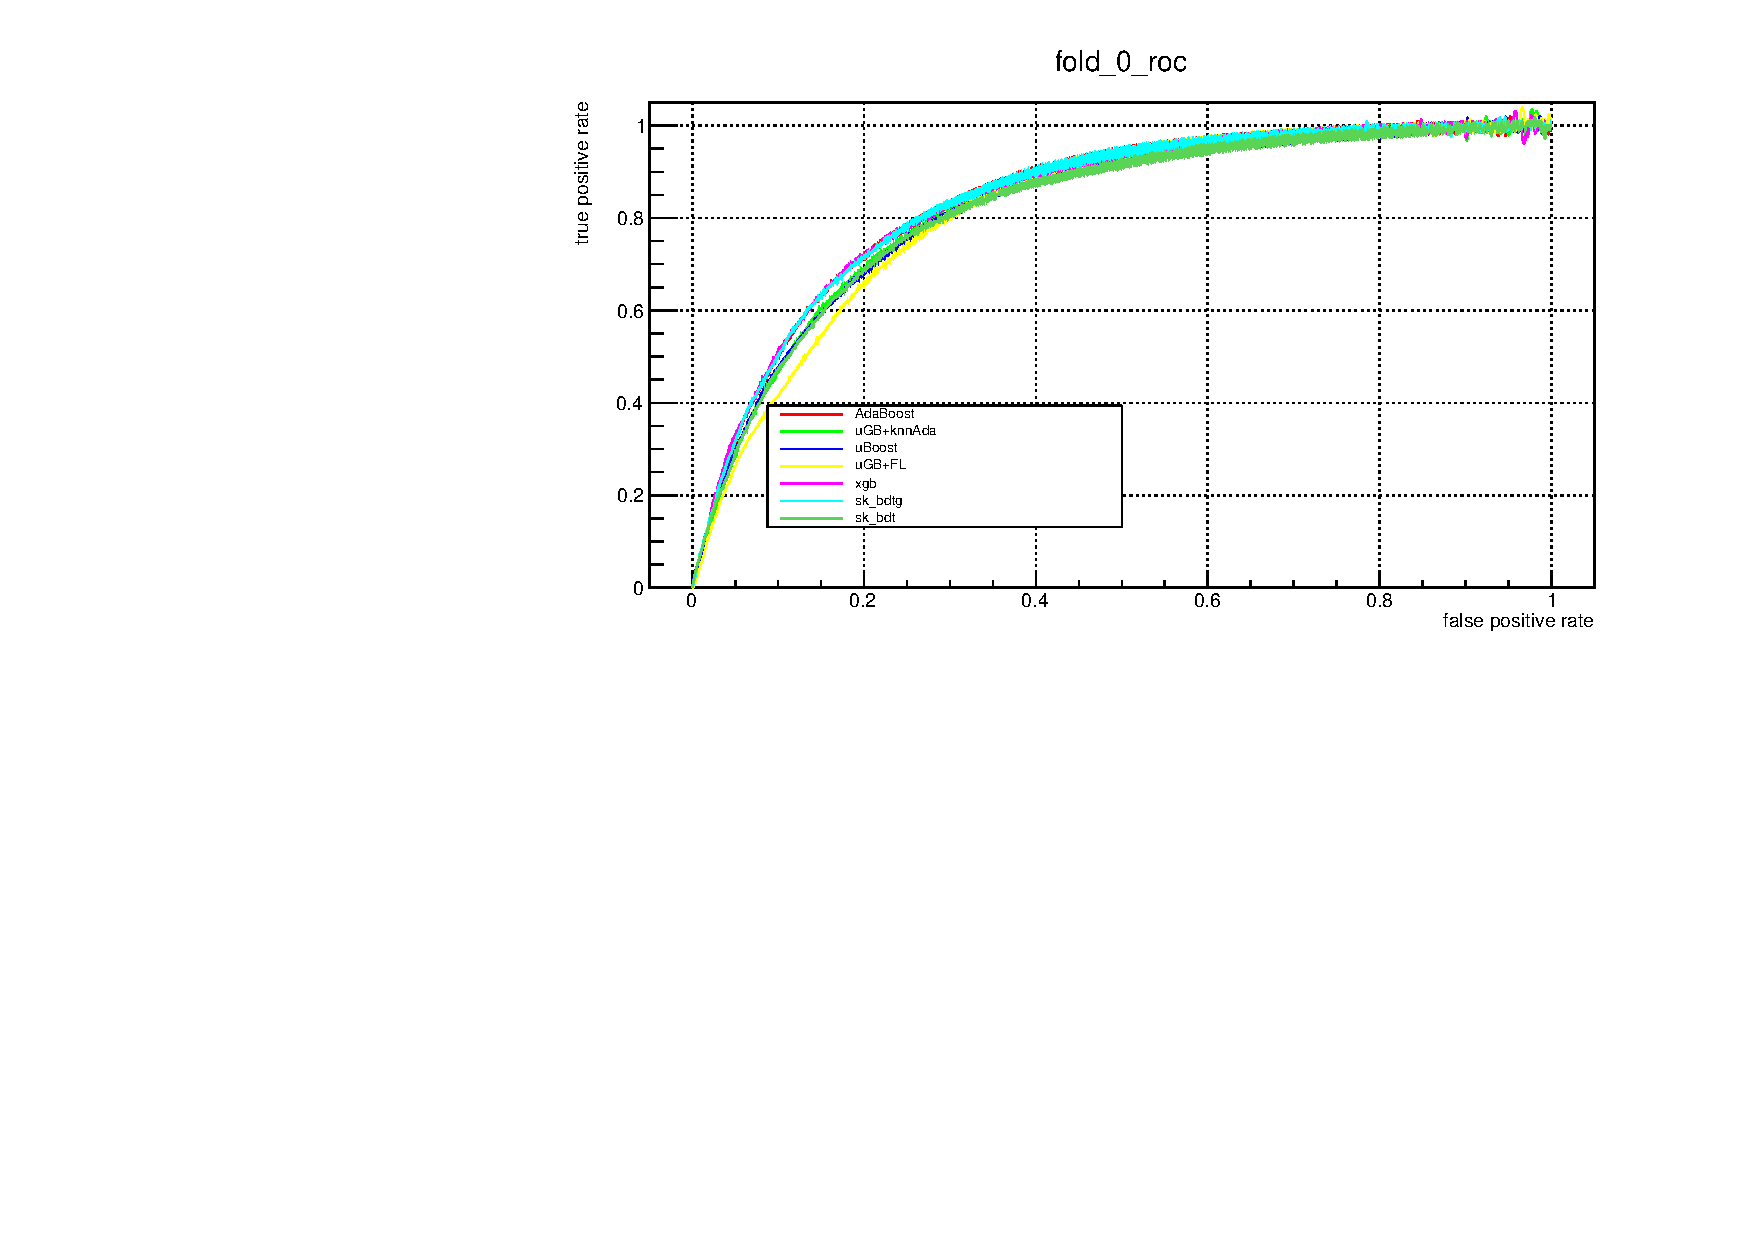
\includegraphics[width=0.8\textwidth]{roc/fold_0_roc.pdf}
 \caption{ROC curve of the first fold. One can see that all the classifiers are competetive in terms of classifing correctly}
 \label{fig:roc}
\end{figure}
The next step is to check for unwanted correlations, only the correlations with the mass are shown here. The others can be found in appendix \ref{app:corr}.
\begin{figure}[H]
 \centering
 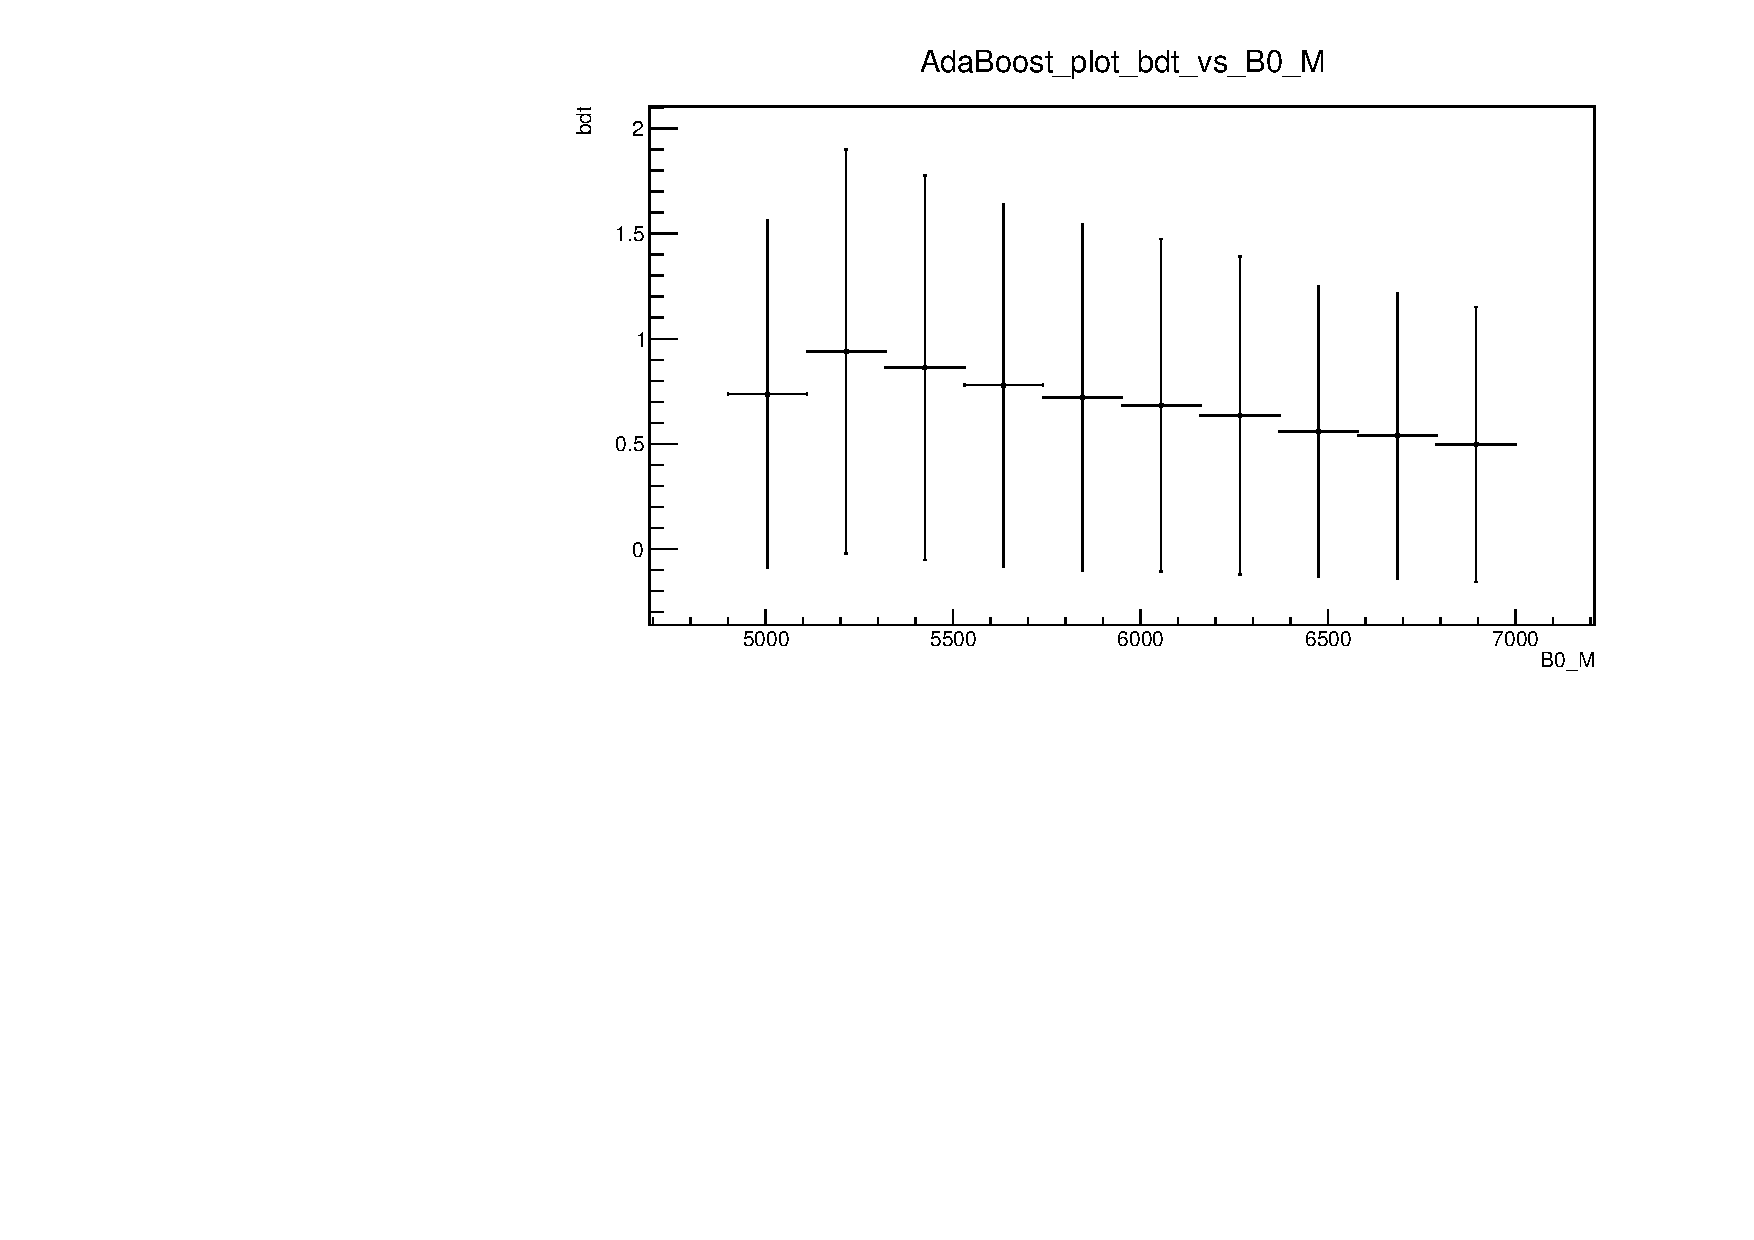
\includegraphics[width=0.5\textwidth]{plots/AdaBoost_plot_bdt_vs_B0_M}
 \caption{This plot shows the correltation between the bdt decision of the AdaBoost classifier and the $B_0$ mass. There is clearly a correlation starting from the second bin from the left.}
 \label{fig:AdaB0M}
\end{figure}

\begin{figure}[H]
 \centering
 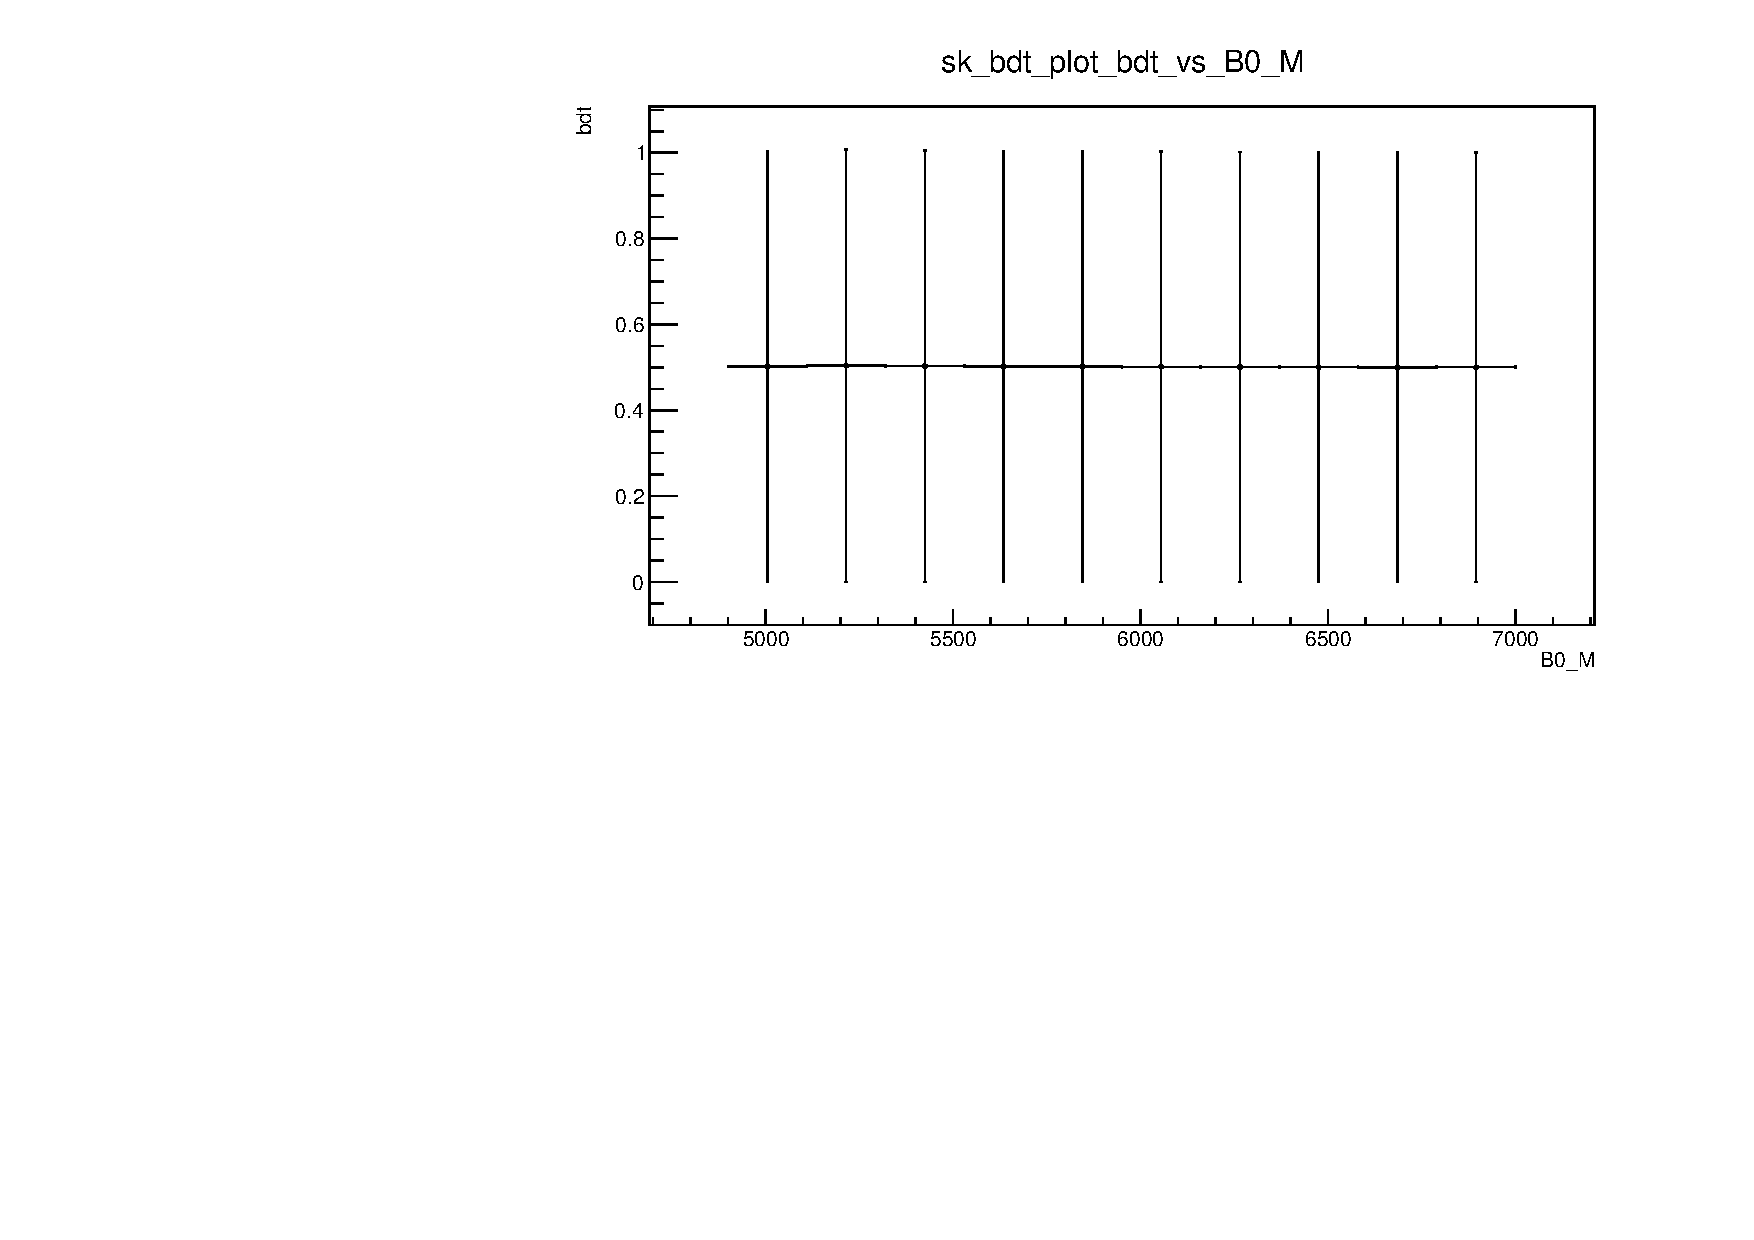
\includegraphics[width=0.5\textwidth]{plots/sk_bdt_plot_bdt_vs_B0_M}
 \caption{This plot shows the correltation between the bdt decision of the sk\_bdt classifier and the $B_0$ mass. There is no correlation.}
 \label{fig:skbdtB0M}
\end{figure}

\begin{figure}[H]
 \centering
 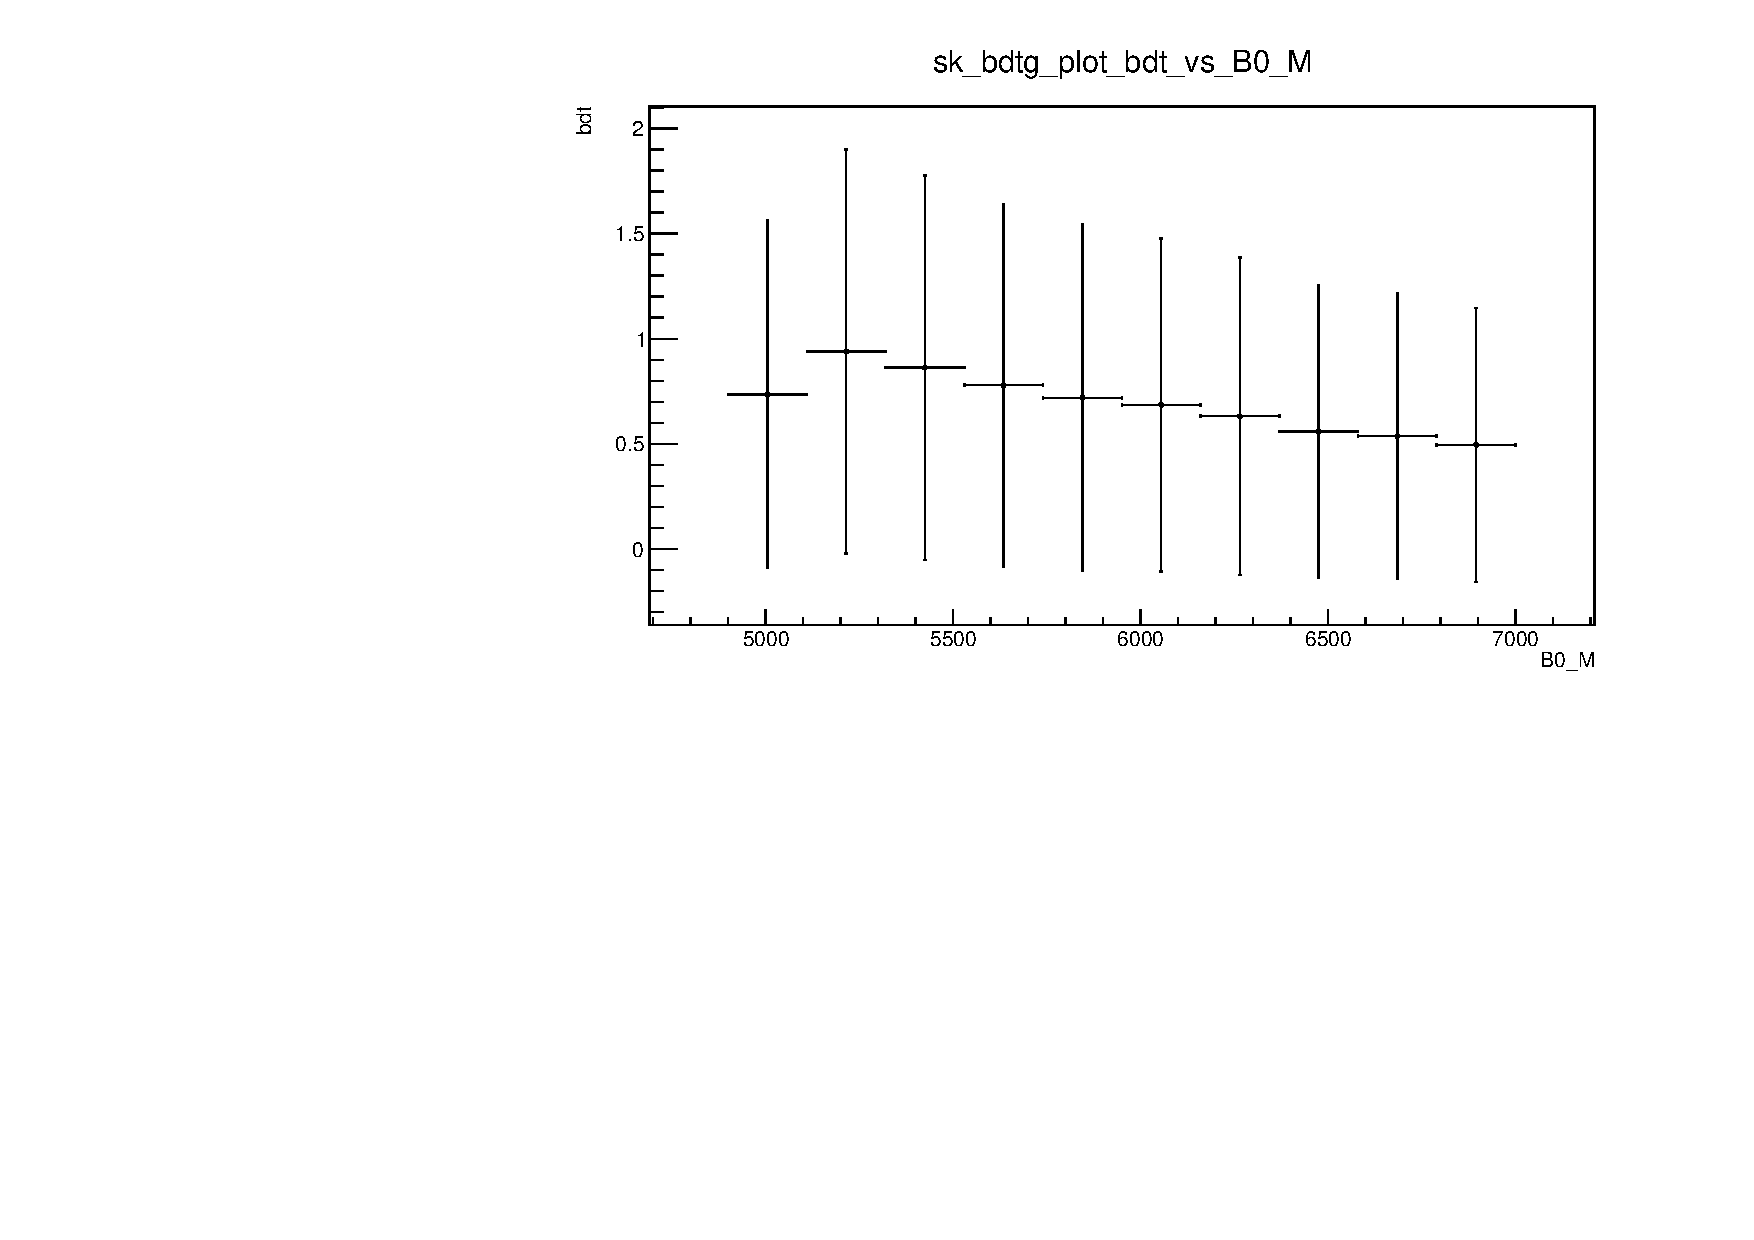
\includegraphics[width=0.5\textwidth]{plots/sk_bdtg_plot_bdt_vs_B0_M}
 \caption{This plot shows the correltation between the bdt decision of the sk\_bdtg classifier and the $B_0$ mass. There is clearly a correlation starting from the second bin from the left.}
 \label{fig:skbdtgB0M}
\end{figure}

\begin{figure}[H]
 \centering
 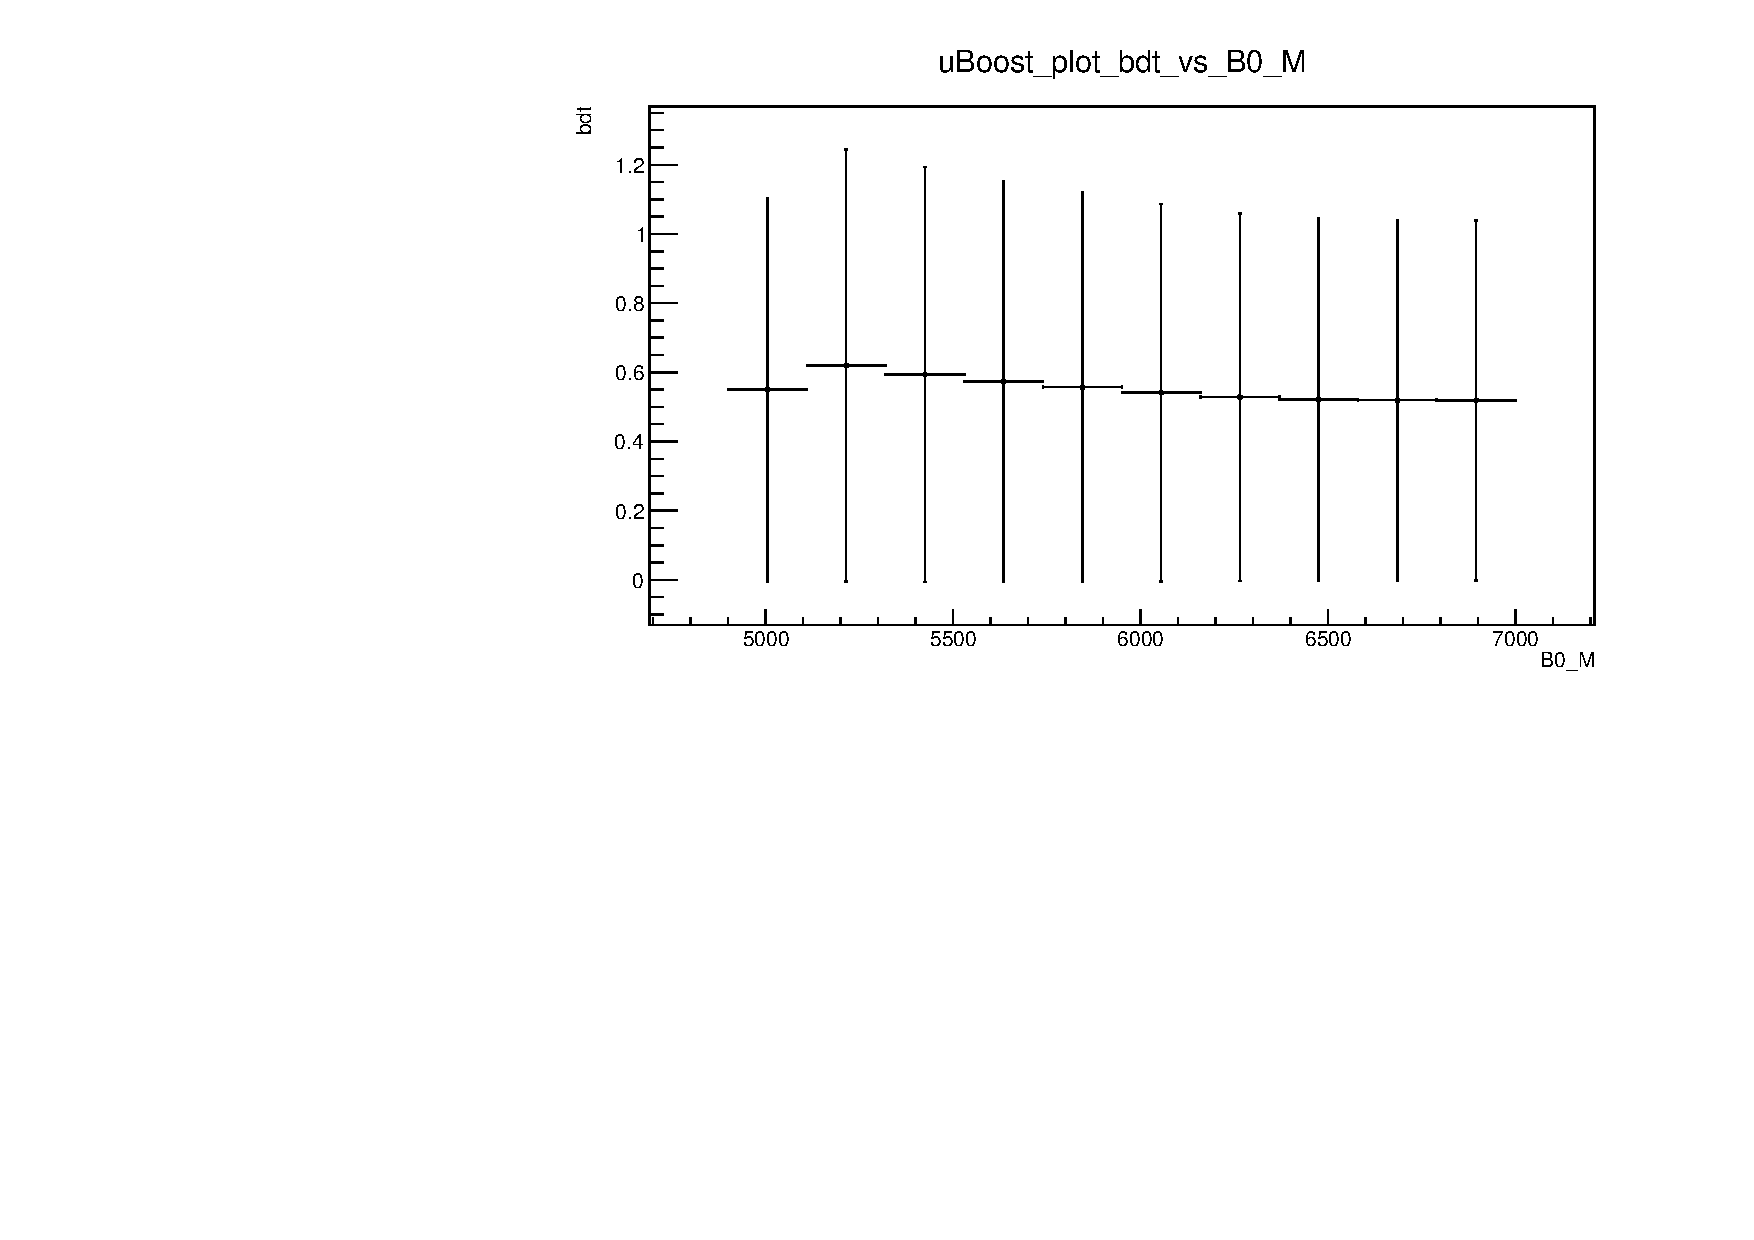
\includegraphics[width=0.5\textwidth]{plots/uBoost_plot_bdt_vs_B0_M}
 \caption{This plot shows the correltation between the bdt decision of the uBoost classifier and the $B_0$ mass. There is just a very small correlation compared to other classifiers.}
 \label{fig:uBoostB0M}
\end{figure}

\begin{figure}[H]
 \centering
 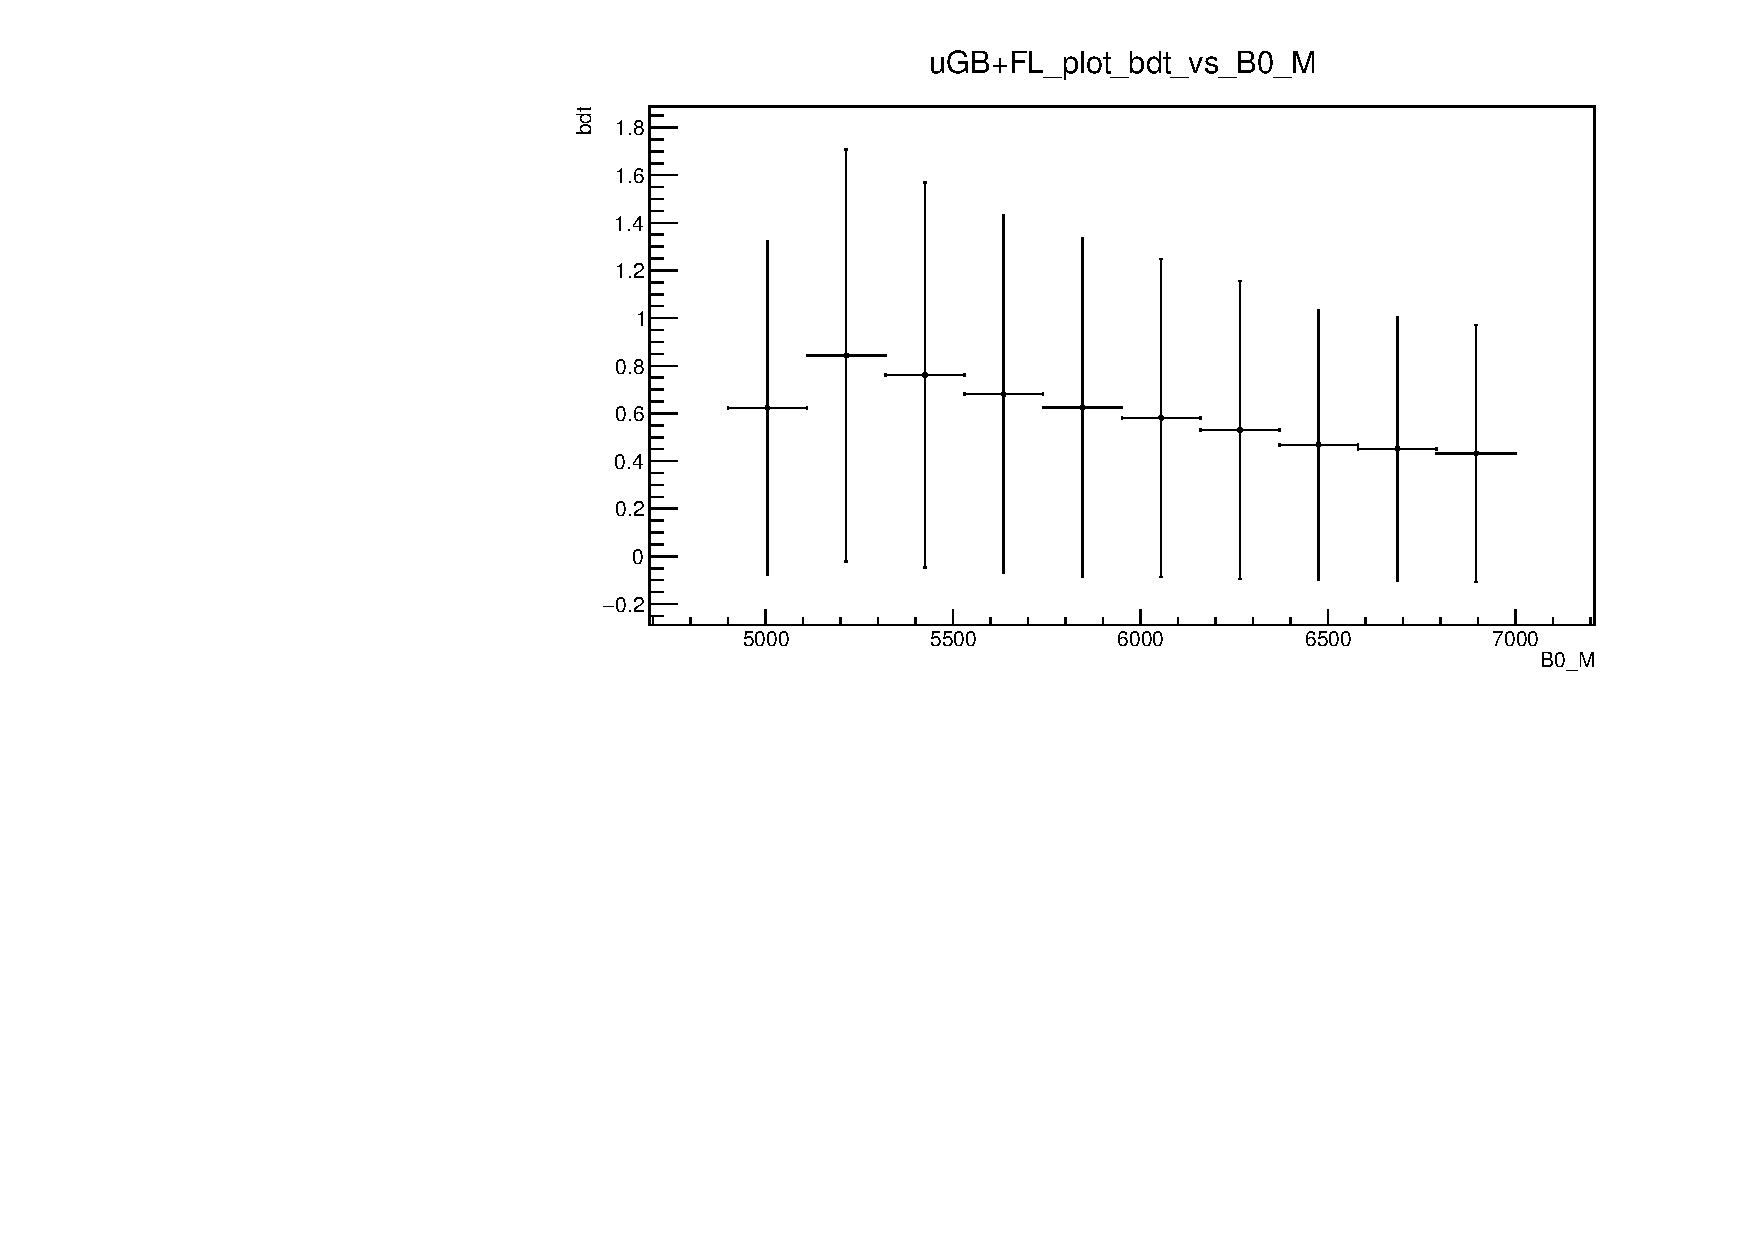
\includegraphics[width=0.5\textwidth]{plots/uGB+FL_plot_bdt_vs_B0_M}
 \caption{This plot shows the correltation between the bdt decision of the uGB+FL classifier and the $B_0$ mass. There is clearly a correlation starting from the second bin from the left.}
 \label{fig:uGB+FLB0M}
\end{figure}

\begin{figure}[H]
 \centering
 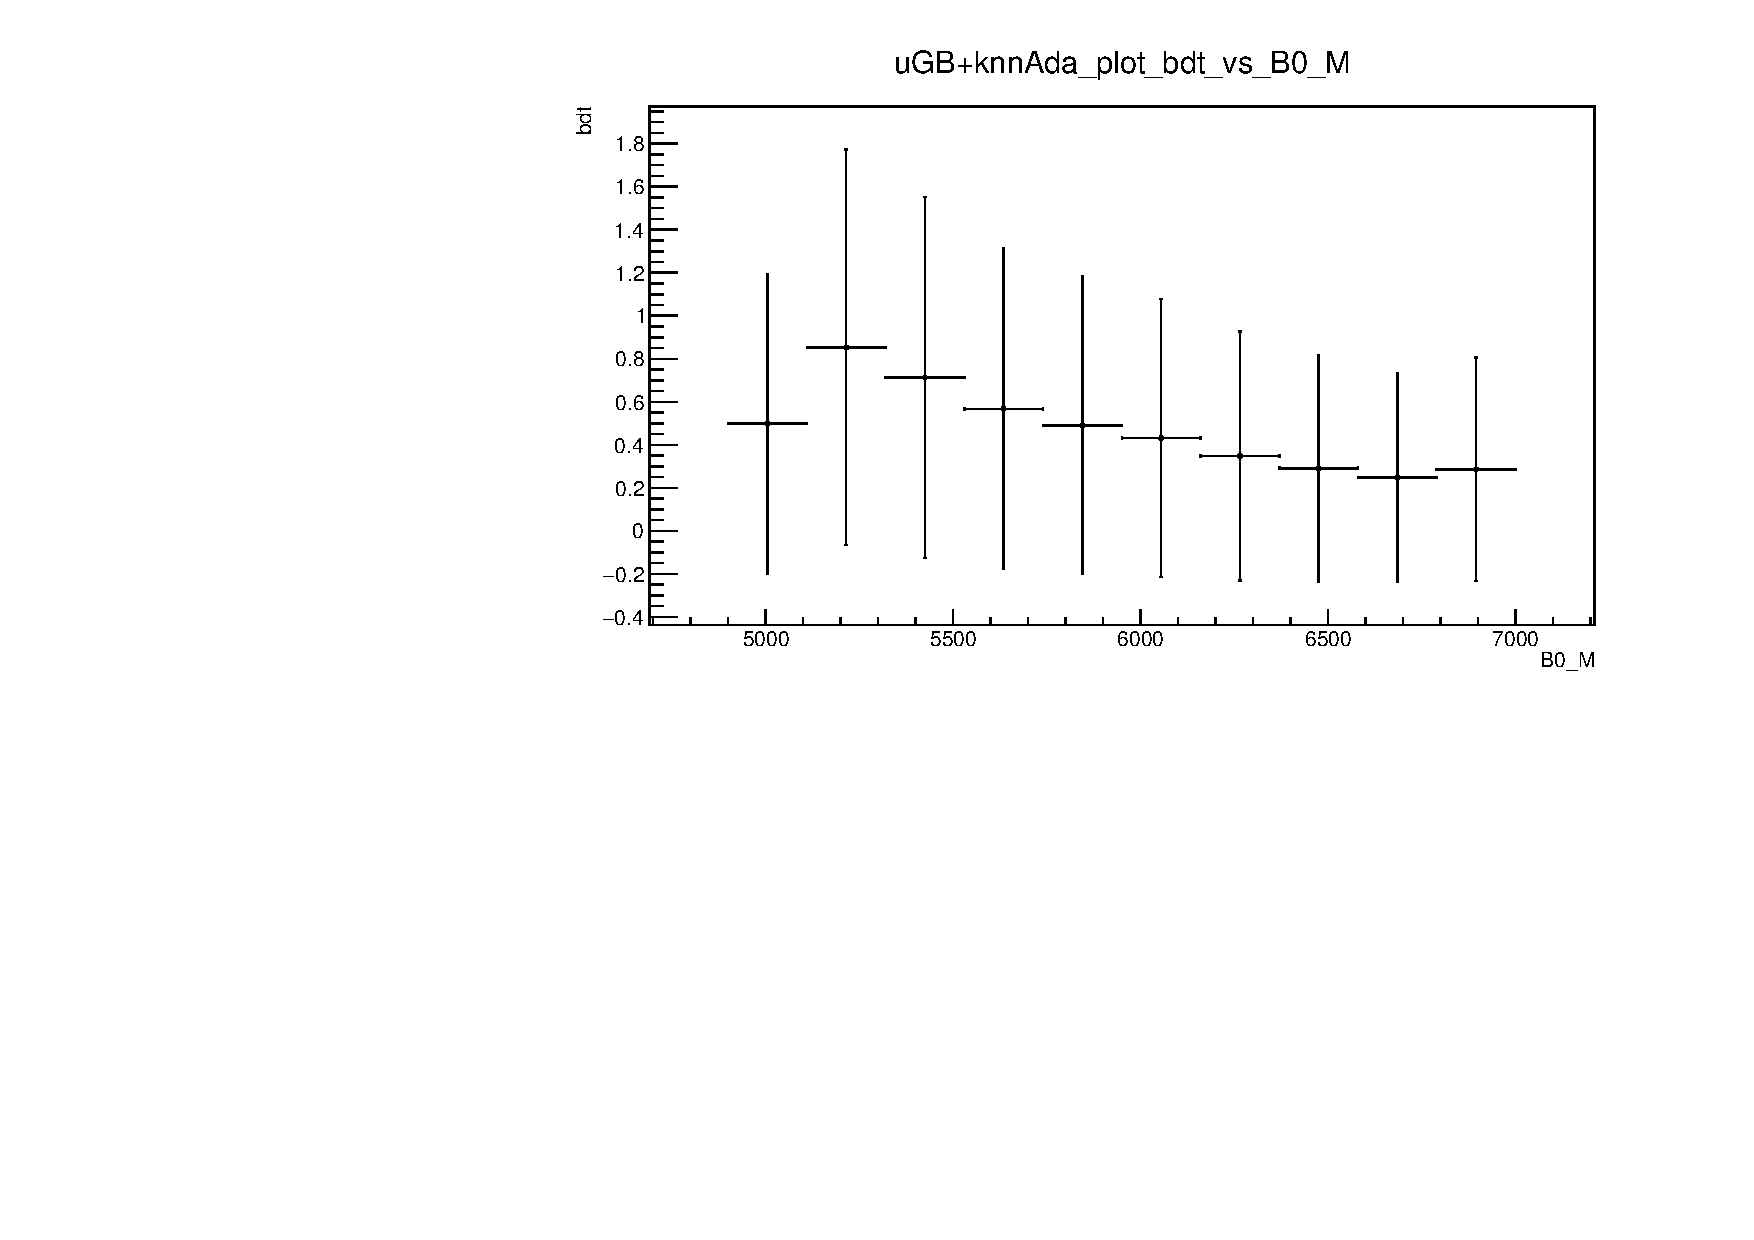
\includegraphics[width=0.5\textwidth]{plots/uGB+knnAda_plot_bdt_vs_B0_M}
 \caption{This plot shows the correltation between the bdt decision of the uGB+knnAda classifier and the $B_0$ mass. There is clearly a correlation starting from the second bin from the left.}
 \label{fig:uGB+knnAdaB0M}
\end{figure}

\begin{figure}[H]
 \centering
 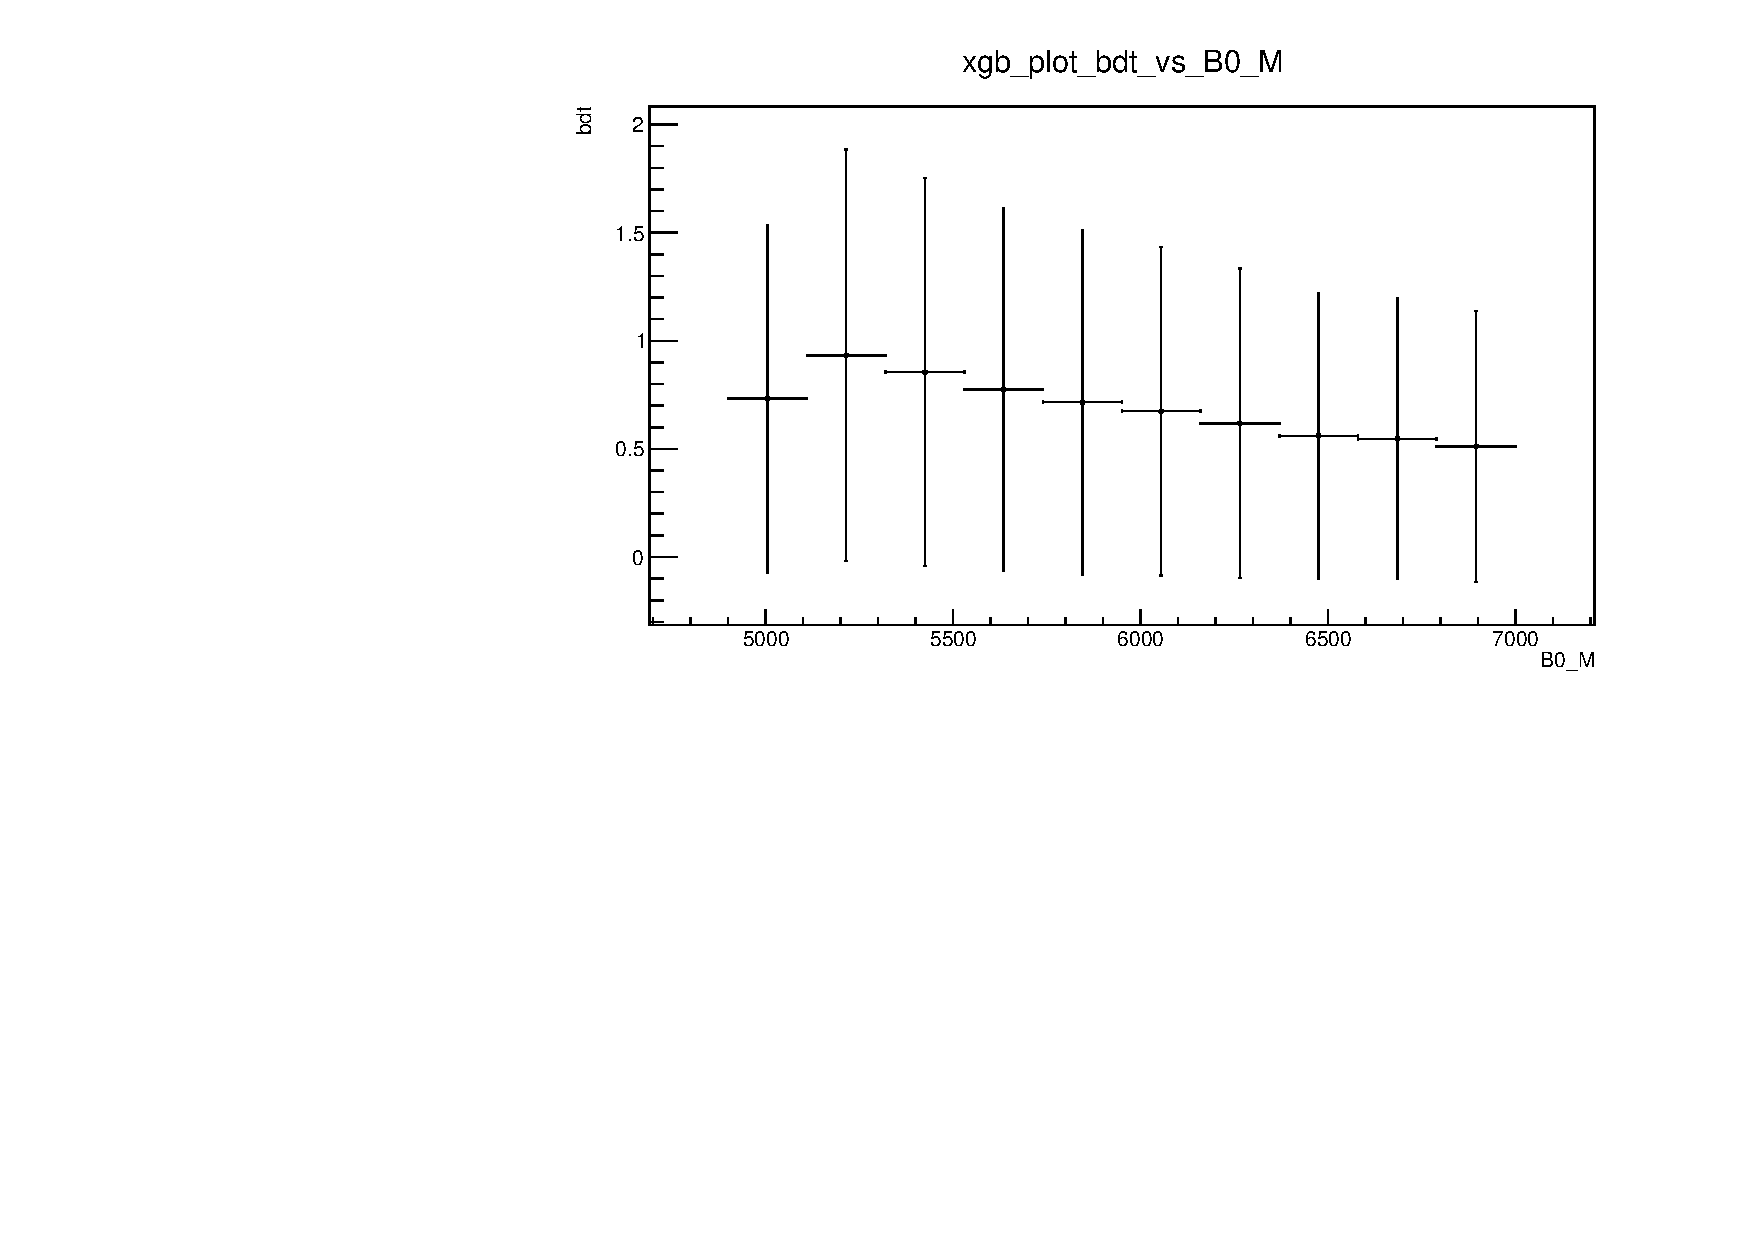
\includegraphics[width=0.5\textwidth]{plots/xgb_plot_bdt_vs_B0_M}
 \caption{This plot shows the correltation between the bdt decision of the xgb classifier and the $B_0$ mass. There is clearly a correlation starting from the second bin from the left.}
 \label{fig:xgbB0M}
\end{figure}

The two classifers with the least correlation are the sk\_bdt and the uBoost classifers. Therfore they were used to do the seperation between signal and background in the $B$ $\rightarrow$ $K^{*}$ $\mu$ $\mu$ data.

\subsection{SPlot}

\subsubsection{Likelihood method}
Consider an analysis of a data sample, which consists of several types of events. These types represent signal components and background components, for example from different experiments. The log-liklihood of such a data sample is expressed as:
\begin{align}
 L = \sum_{i=1}^{N} \ln \left[ \sum_{j=1}^{N_S} N_j f_j (y_i) \right] - \sum_{i=j}^{N_S} N_j \label{eq:L}
\end{align}

\begin{itemize}
 \item $N$ = total number of events \\
 \item $N_S$ = number of types \\
 \item $N_i$ = expected average number of events for type $i$ \\
 \item $y$ = set of diciminating variables \\
 \item $f_j$ = PDF of the $i$th type \\
 \item $f_j(y_i)$ = value of PDF for event $y_i$ \\
 \item $x$ = control variable, not a part of $L$ by construction
\end{itemize}
The yields $N_i$ and the free parameters of the PDF are obtained by maximizing the above log-likelihood (eq \ref{eq:L}).

\subsubsection{$_{in} Plot$ technique}
Consider a varibale x which can be expressed as a function of the dicriminating variables y used in the fit. Furthermore a fit has been performed to determine the yields $N_i$ for all types. From the knowledge of the PDF and the values of $N_i$ a naive weight can be defined as:
\begin{align}
 P_n(y_i) = \frac{N_n f_n(y_i)}{\sum_{k=1}^{N_s} N_k f_k(y_i)} \label{eq:P_n}
\end{align}
which will leed to the x-distribution $\tilde{M}_n$ defined by:
\begin{align}
 N_n \tilde{M}_n (\bar{x}) = \sum_{i \subset \delta x} P_n (y_i) \label{eq:Mn}
\end{align}
where sum $\sum_{i \subset \delta x}$ contains alle events for which $x_i$ lies in the interval centered on $\bar{x}$ and of total width $\delta x$.
Therefor $N_n \tilde{M}_n (\bar{x}) \delta x$ is the x-distribution of the histogrammed events, using the weights of eq \ref{eq:P_n}.
With this procedure one can on average reproduce the true distribution $\textbf{M}_n(x)$. One can even replace the sum in eq \ref{eq:Mn} by an integral:
\begin{align}
 \left \langle \sum_{i \subset \delta x} \right \rangle \rightarrow \int dy \sum_{j=1}^{N_s} N_j f_j (y) \delta (x(y) - \bar{x}) \delta x \label{eq:average}
\end{align}
Furthermore through identifying the number of events $N_i$ from the fit one gets:
\begin{align}
 \langle N_n \rangle \tilde{M}_n (\bar{x}) & = \int dy \sum_{j=1}^{N_s} N_j f_j (y) \delta (x(y) - \bar{x}) P_n (y)                                               \\
                                           & = \int dy \sum_{j=1}^{N_s} N_j f_j (y) \delta (x(y)- \bar{x}) \cdot \frac{N_n f_n (y)}{\sum_{k=1}^{N_s} N_k f_k (y)} \\
                                           & = N_n \int dy \delta (x(y) - \bar{x}) f_n (y)                                                                        \\
                                           & = N_n \textbf{M}_n(\bar{x}) \label{eq:N_nM_n}
\end{align}
One can see that the sum over enents of the daive weight $P_n$ provides a direct estimate of the x-distribution for the nth type.
But this procedure has a major drawback, since x is correlated to y, the PDFs of x enter implicity in the definition of the naive weight. Therfor the $\tilde{M}_n$ distributions are a bad estimate for the quality of the fit, since the these distributions are biased in a difficult way, when the PDFs $f_i(y)$ are not accurate. \\
Consider for example a data sample where one of the types has events on the tail of the x-distribution. Such events require the true ditribution to account for the tail. But since the events are averaged the weights on the tail are going to be very small missing those events in the extimated true distribution. Only the core of the x-distribution can be examined with $_{in} Plots$.


\subsubsection{$_{S} Plot$ technique}
In the previous section it was shown that if a variable x belongs to a set y of discriminating varibales, one can reconstruct the expected x distribution.
Consider now two sets of variables $x$ and $y$, where x does not belong to y and which are uncorrelated , hence the total PDFs $f_i (x,y)$ all factorize into products $\textbf{M}_i (x) f_i(y)$.
The equation \ref{eq:N_nM_n} does not hold anymore because, when summing over the events the x-PDFs $\textbf{M}_j(x)$ appear:

\begin{align}
 \langle N_n \rangle \tilde{M}_n (\bar{x}) & = \int \int dy dx \sum_{j=1}^{N_s} N_j \textbf{M}_j (x) f_j (y) \delta (x- \bar{x}) P_n \label{eq:M_nX}                    \\
                                           & = \int dy \sum_{j=1}^{N_s} N_j \textbf{M}_j (\bar{x}) f_j(y) \frac{N_n f_n(y)}{\sum_{k=1}^{N_s} N_k f_k(y)}                \\
                                           & = N_n \sum_{j=1}^{N_s} \textbf{M}_j (\bar{x}) \left( N_j \int dy \frac{f_n(y) f_j(y)}{\sum_{k=1}^{Ns} N_k f_k (y)} \right) \\
                                           & \neq N_n \textbf{M}_n (\bar{x}).
\end{align}

The correction term

\begin{align}
 N_j \int dy \frac{f_n (y) f_j (y)}{\sum_{k=1}^{N_s} N_k f_k(y)}
\end{align}
is not identical to the kroenecker delta $\delta_{jn}$. In fact the $N_n \tilde{M}_n$ distribution obtained by the naive weight is a linear combination of the true distribution $\textbf{M}_j$. \\
To go forward one has to realize that the correction term is related to the inverse of the covariance matrix, given by the second derivatives of $-L$, after the minimization.
\begin{align}
 \textbf{V}_{nj}^{-1} = \frac{\partial^2 (-L)}{\partial N_n \partial N_j} = \sum_{i=1}^{N} \frac{f_n(y_i) f_j(y_i)} {\left( \sum_{k=1}^{N_s} N_k f_k(y_i) \right)^2}
\end{align}
If one averages and is replacing the sum over events by intergals (eq \ref{eq:average}) the varaince matrix reads:
\begin{align}
 \langle \textbf{V}_{nj}^{-1} \rangle & = \int \int dy dx \sum_{e=1}^{N_s} N_e \textbf{M}_e(x) f_e(y) \frac{f_n(y) f_j(y)}{ \left( \sum_{k=1}^{N_s} N_k f_k(y) \right)^2}       \\
                                      & = \int dy \sum_{e=1}^{N_s} N_e f_e(y) \frac{f_n(y) f_j(y)}{ \left( \sum_{k=1}^{N_s} N_k f_k(y) \right)^2} \cdot \int dx \textbf{M}_l(x) \\
                                      & = \int dy \frac{f_n (y) f_j (y)}{\sum_{k=1}^{N_s} N_k f_k(y)}
\end{align}
Therefor equation \ref{eq:M_nX} can be rewritten as:
\begin{align}
 \langle \tilde{M}_n (\bar{x}) \rangle = \sum_{j=1}^{N_s} \textbf{M}_j (\bar{x}) N_j \langle \textbf{V}_{nj}^{-1} \rangle .
\end{align}
To get the distribution of intrest one has to invert this matrix equation:
\begin{align}
 N_n \textbf{M}_n(\bar{x}) = \sum_{j=1}^{N_s} \langle \textbf{V}_nj \rangle \langle \tilde{M}_j (\bar{x}) \rangle
\end{align}
The true distribution of $x$ can still be reconstructed using the naive weight (eq \ref{eq:P_n}), through a linear combination of $_{in} Plots$. In other words: When x does not belong to the set y, the weights are not given by equation \ref{eq:P_n}, they are given by a covariance-weighted quantity called sWeight defined by:
\begin{align}
 _s P_n(y_i) = \frac{\sum_{j=1}^{N_s} \textbf{V}_nj f_j(y_i)} {\sum_{k=1}^{N_s} N_k f_k (y_i)} \label{eq:sWeight}
\end{align}
With the sWeights on can obtain the distribution of the x variable by histogramming the $_s Plot$:
\begin{align}
 N_n { }_{s} \tilde{M}_n (\bar{x}) \delta x = \sum_{i \subset \delta x} { }_{s} P_n (y_i) \label{eq:sPlot2}
\end{align}
On average it reproduced the true distribution:
\begin{align}
 \langle N_n { }_s \tilde{M}_n (x) \rangle = N_n \textbf{M}_n (x)
\end{align}
In the case were x is significantly correlated with y, the $_s Plots$ from equation \ref{eq:sPlot2} connt be compared with the pure distributions of the various types. To solve that problem one can perform a Monte Carlo simulation of the procedure and obtain the expected distributions to which the $_s Plots$ should be compared with. \\
For more information on $_s Plots$ consider reading \cite{bib:sPlot}.


\subsection{Reweighting}
The infomation needed in an analysis is not all contained inside the data. For example efficiencies can not be recorded by a detector. But they can be simulated by a Monte Carlo simulation of the particle decay. The problem is that the simulation has to be the same as data to get the correct answers. Since resimulating everything with different parameters until one hits the data distribution would take too much resources. One can simply reweight the simulation to match the data. As an initial weight the sWeights see equation \ref{eq:sWeight} are used. The parameters used to reweight the MC samples are applied in the following order: 'nTracks', '$B_0$ $p_T$' and the quality of the $K \pi \mu \mu$ vertex. The new weights derived by the difference in data and simulation of these parameters are used to weight all the MC samples. For this analysis the MC and Data of the $K^* \rightarrow J/ \Psi K^{*0}$ are used, because it is a very clean channel.




\section{RooMCMarkovChain}
RooMCMarkovChain is a new class for the ROOT Data Analysis Framework, which can be used to for fits and presents a alternative to the brodly used MINUIT algorithm. RooMCMarkovChain uses a metropolis algorithm as a minimizer for the negative log likelihood function. The metropolis algorithm is based ona Monte Carlo Markov Chain and can therfore easily be scaled to multidimensional parameter space and moreover, such kind of algorithms can easily be parallelized.

\subsection{Monte Carlo Markov Chain (MCMC)}
A Markov Chain is a random process which undergoes several states. From each state there is a probability ditribution to change into another state or to stay. Most important i the asumption that every next step just depends on the current state.
The figure \ref{fig:MCMC} illustrates the behavior of such a Markov Chain.

\begin{figure}[H]
  \centering
  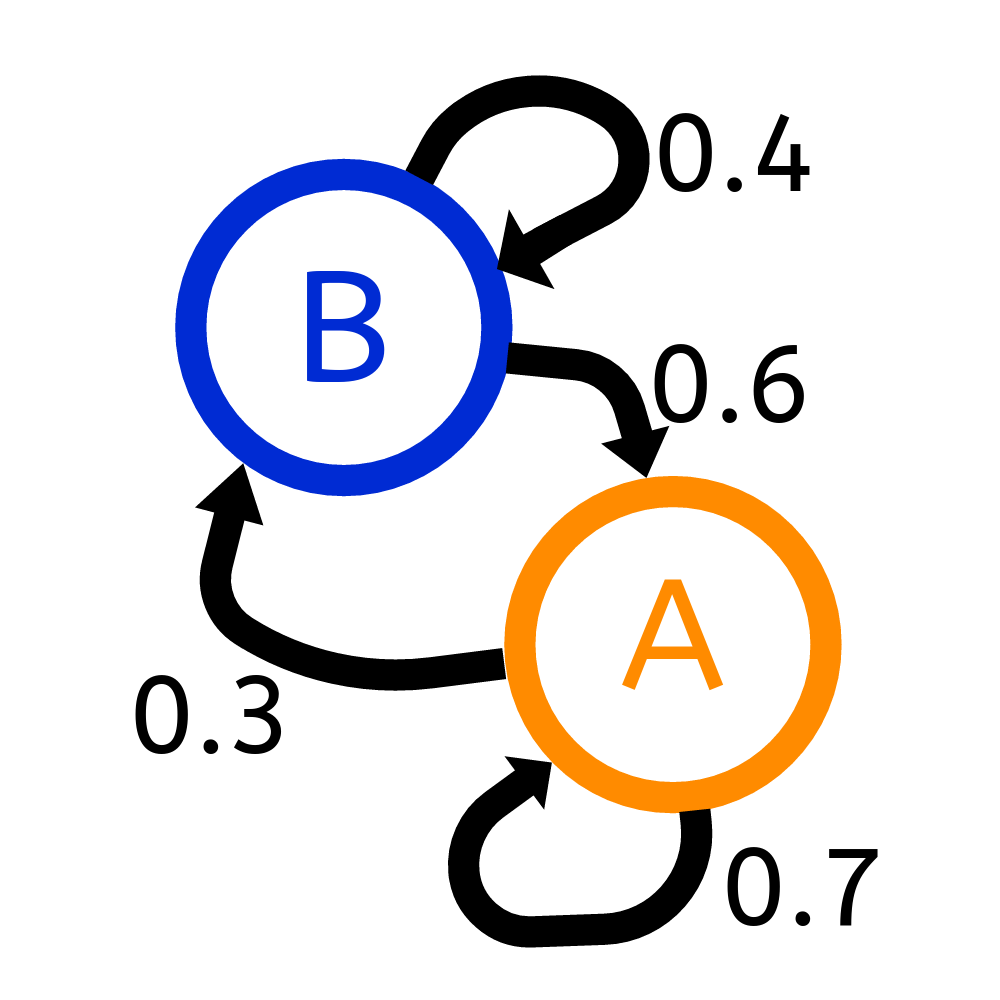
\includegraphics[width=0.3\textwidth]{MCMC_Chain}
  \caption{Illustration of states and the probability distribution to change or the stay in a state of a Monte Carlo Markov Chain. In state A there is a 0.3 probability to change into state B and a 0.7 probability to stay in state A.}
  \label{fig:MCMC}
\end{figure}

\subsection{Metropolis Hastings}


Metropolis Hastings is a so called Monte Carlo updater. It updates the probabillity distribution when a change of states is proposed. That is very usefull in the cases where the states are not discrete like in figure \ref{fig:MCMC} but continous. Suppose that a specified distribution has unnormalized density $h$. The Metopolis Hastings update does the following:
\begin{enumerate}
  \item The current state x is proposed to move to another state y with a conditional probability given x denoted as $q(x,\cdot)$.
  \item The Hastings ratio is calculated:
  \begin{align}
    r(x,y) = \frac{h(y) \cdot q(y,x)}{h(x) \cdot q(x,y)} \label{eq:r(x,y)}
  \end{align}
  \item The proposed move to y is accepted with the probability $a(x,y)$:
  \begin{align}
    a(x,y) = min(1,r(x,y))
  \end{align}
\end{enumerate}

This principle is used in the RooMCMarkovChain class to minimize the negative log likelihood function. In detail a robust adaptive Metrpolis hastings process is implemented. It is defined as:
\begin{enumerate}
  \item  Compute next proposed state $Y_n$ as a random change from the current state $X_{n-1}$:
  \begin{align*}   Y_n &\equiv X_{n-1} + S_{n-1} U_n    \end{align*}
  , where $U_n$ is an independent random vector.
  \item With the probability $\alpha_n$ the proposal is accepted and $X_n = Y_n$. Otherwise the proposal is rejected and $X_n = X_{n-1}$
  \begin{align*}  \alpha_n &\equiv min\{ 1, r(X_{n-1},Y_n) \} \end{align*}
  , where $r$ is the hastings ratio see equation \ref{eq:r(x,y)}.
  \item compute the lower-diagonal matrix $S_n$ with positive diagonal elements satisfying the equation:
  \begin{align}
    S_n S_n^T = S_{n-1} \left( I + \eta_n(\alpha_n - \alpha_*) \frac{U_n Y_n^T}{||U_n||^2} \right) S_{n-1}^T
  \end{align}
  ,where $I \in R^{dxd}$ is the identity matrix.
\end{enumerate}



\subsection{Features}
 The features of the RooMCMarkovChain class will be shown by fitting the following probability density function (pdf):
\begin{align}
  g(x) = \frac{1}{\sqrt{2 \pi \sigma_1^2}} e^{- \frac{(x-\mu_1)^2}{2 \sigma_1^2}} + f \cdot  \frac{1}{\sqrt{2 \pi \sigma_2^2}} e^{- \frac{(x-\mu_2)^2}{2 \sigma_2^2}} \label{eq:gausspdf}
 \end{align}
It is so called double gaus pdf, which is just the sum of two gaussian pdfs with a fractional parameter $f$.
The result of the fit is compared with the result of the Minuit algorithm:

\begin{figure}[H]
  \centering
  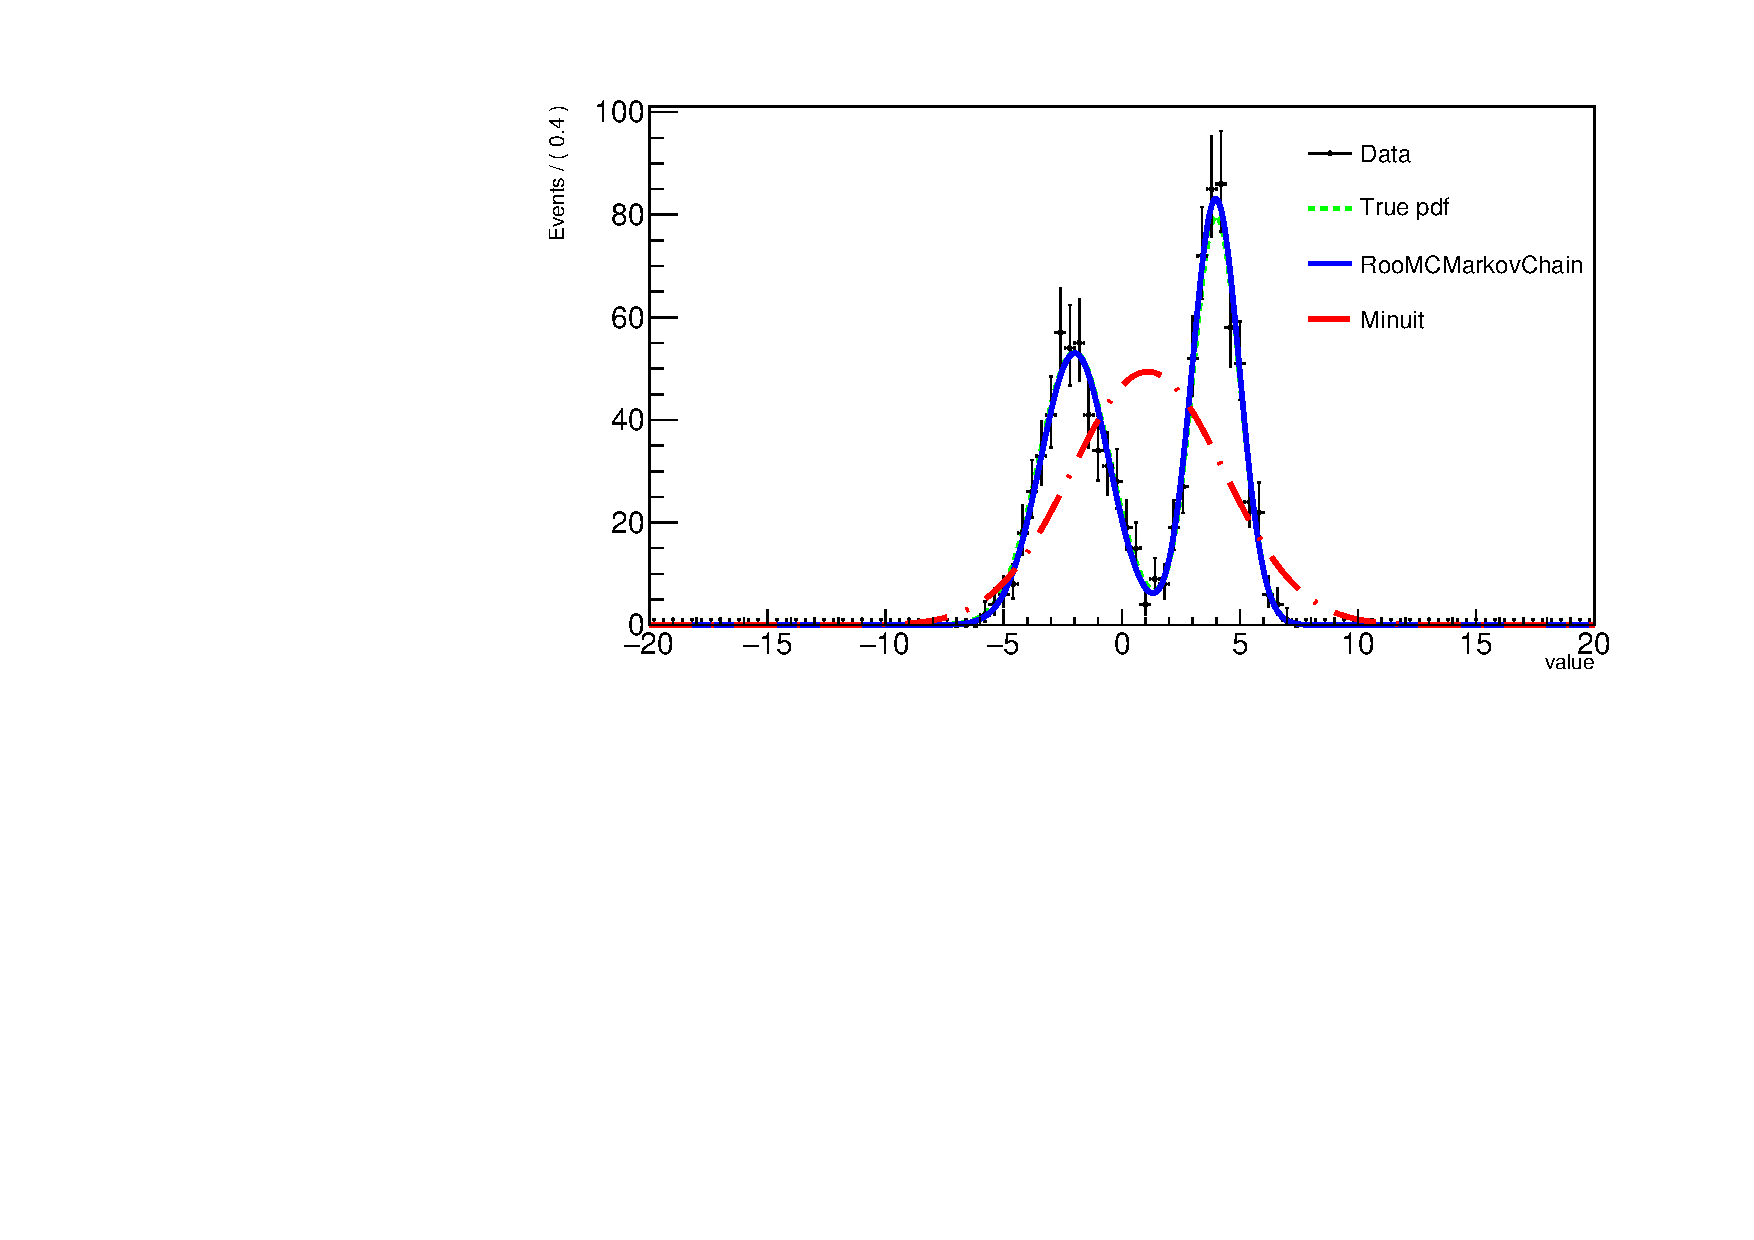
\includegraphics[width=0.8\textwidth]{RooMCMC/twogausfit}
  \caption{Fit of double gaus pdf (see equation \ref{eq:gausspdf}) with RooMCMCarkovchain and with Minuit. The true pdf has the follwing values: $\mu_1 = 4$, $\sigma_1 = 1$, $\mu_2 = -2$, $\sigma_2 = 1.5$ and the fraction $f = 0.5$}
  \label{fig:twogaus}
\end{figure}

The corresponding terminal output gives the estimated parameters with error interval and correlation coefficents of each parameter pair.

\begin{figure}[H]
  \centering
  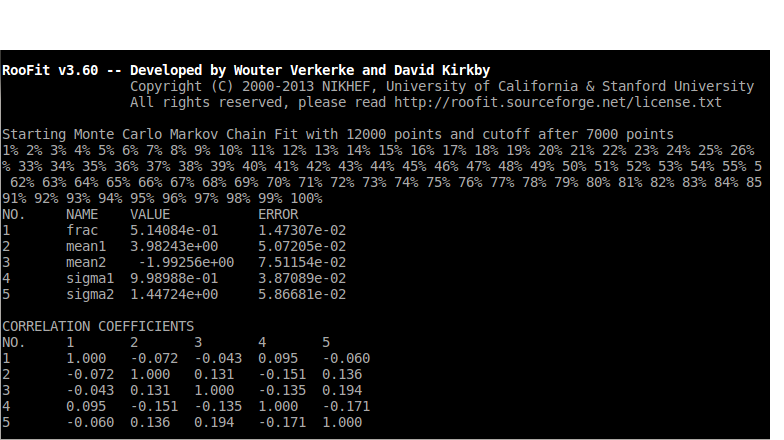
\includegraphics[width=0.8\textwidth]{RooMCMC/terminal_output}
  \caption{Terminal output of the RooMCMarkovChain fit.}
  \label{fig:terminal}
\end{figure}
This gives a good initial overview of results after the fit has finished. The error calculation can be set to assume gaussian or non-gaussian errors.

In addition several other properties of the parameters can be obtainded:
\begin{enumerate}
  \item The 1 dimensional profile of the negative log liklihood function for a given parameter.
  \begin{figure}[H]
    \centering
    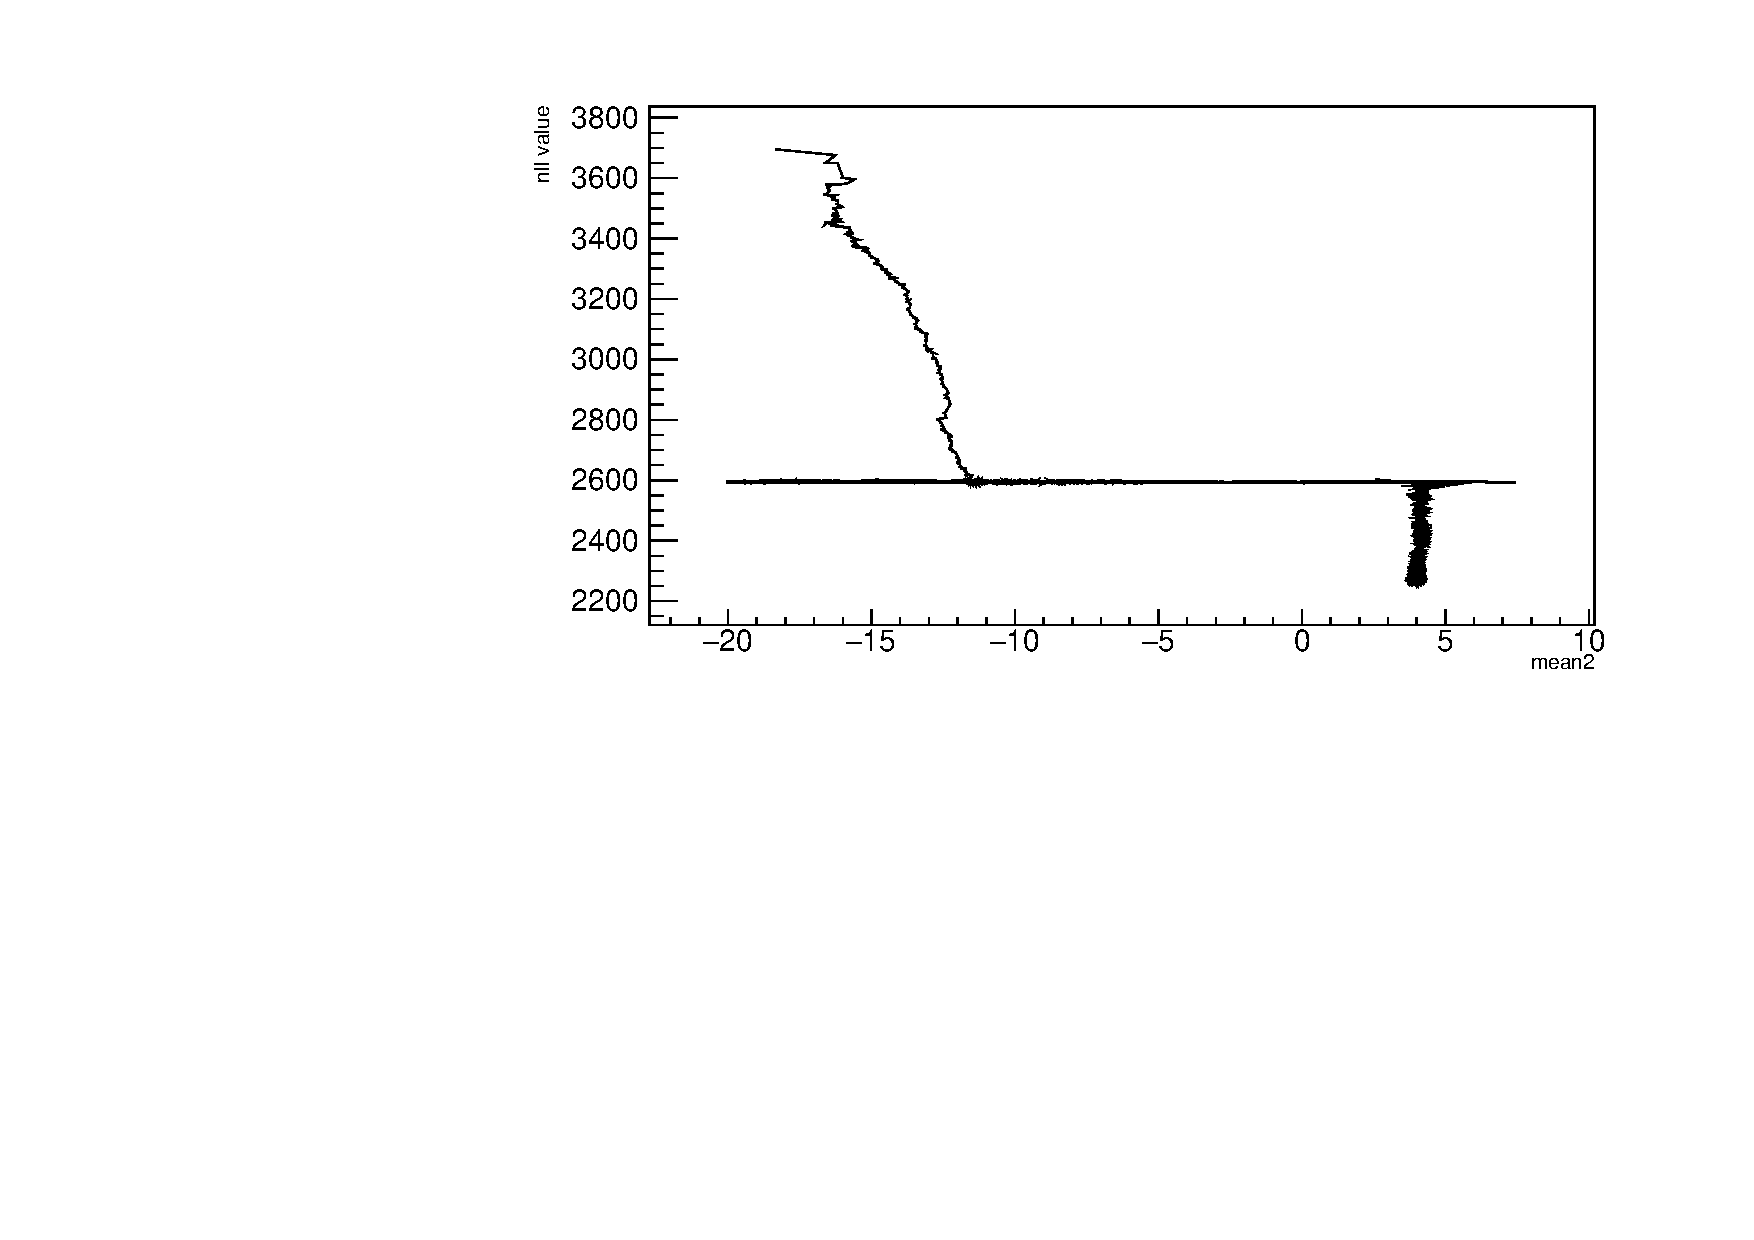
\includegraphics[width=0.8\textwidth]{RooMCMC/walkProfile}
    \caption{Profile of the negative log lilihood function for $\mu_2$ in equation \ref{eq:gausspdf}. There is a local minimum at the nll value of 2600.}
    \label{fig:profile}
  \end{figure}
  From this plot on can see how the algorithm reached the minimum of the negative log likelihood function and if there are local minima. \\


  \item The walk distribution of a given parameter.
  \begin{figure}[H]
    \centering
    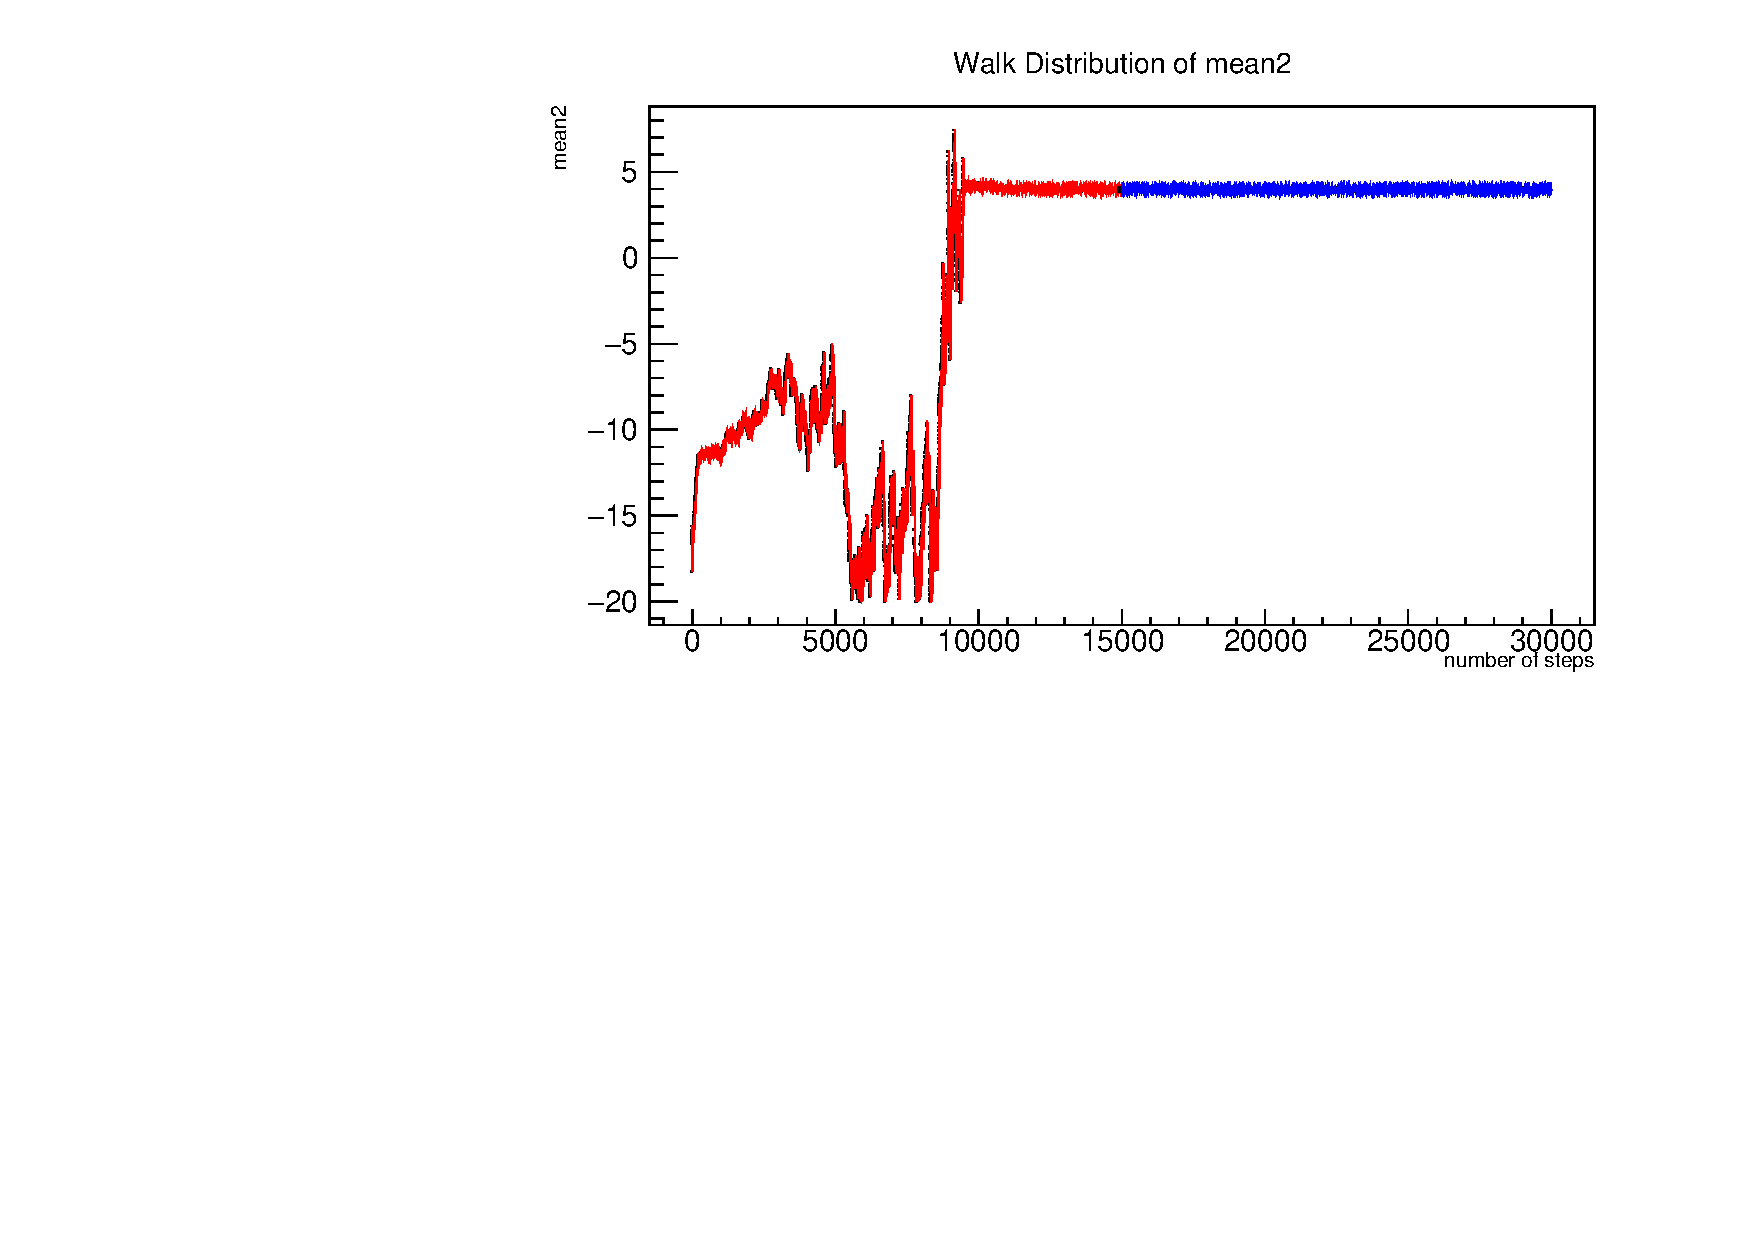
\includegraphics[width=0.8\textwidth]{RooMCMC/walkDis}
    \caption{Walk distribution of $\mu_2$ in equation \ref{eq:gausspdf}. The red points are not considered for the error calculation.}
    \label{fig:walkDis}
  \end{figure}
  This plot is very important for handling the RooMCMarkovChain class. Since the error calculation is based on the variance of the walk distribution, cutting of points in the begginning greatly reduces this variance. The user has to choose how many points are cut off. Plotting the walk distribution of all parameters helps choosing the right amount. \\

  \item The walk distribution of a given parameter as a histogramm.
  \begin{figure}[H]
    \centering
    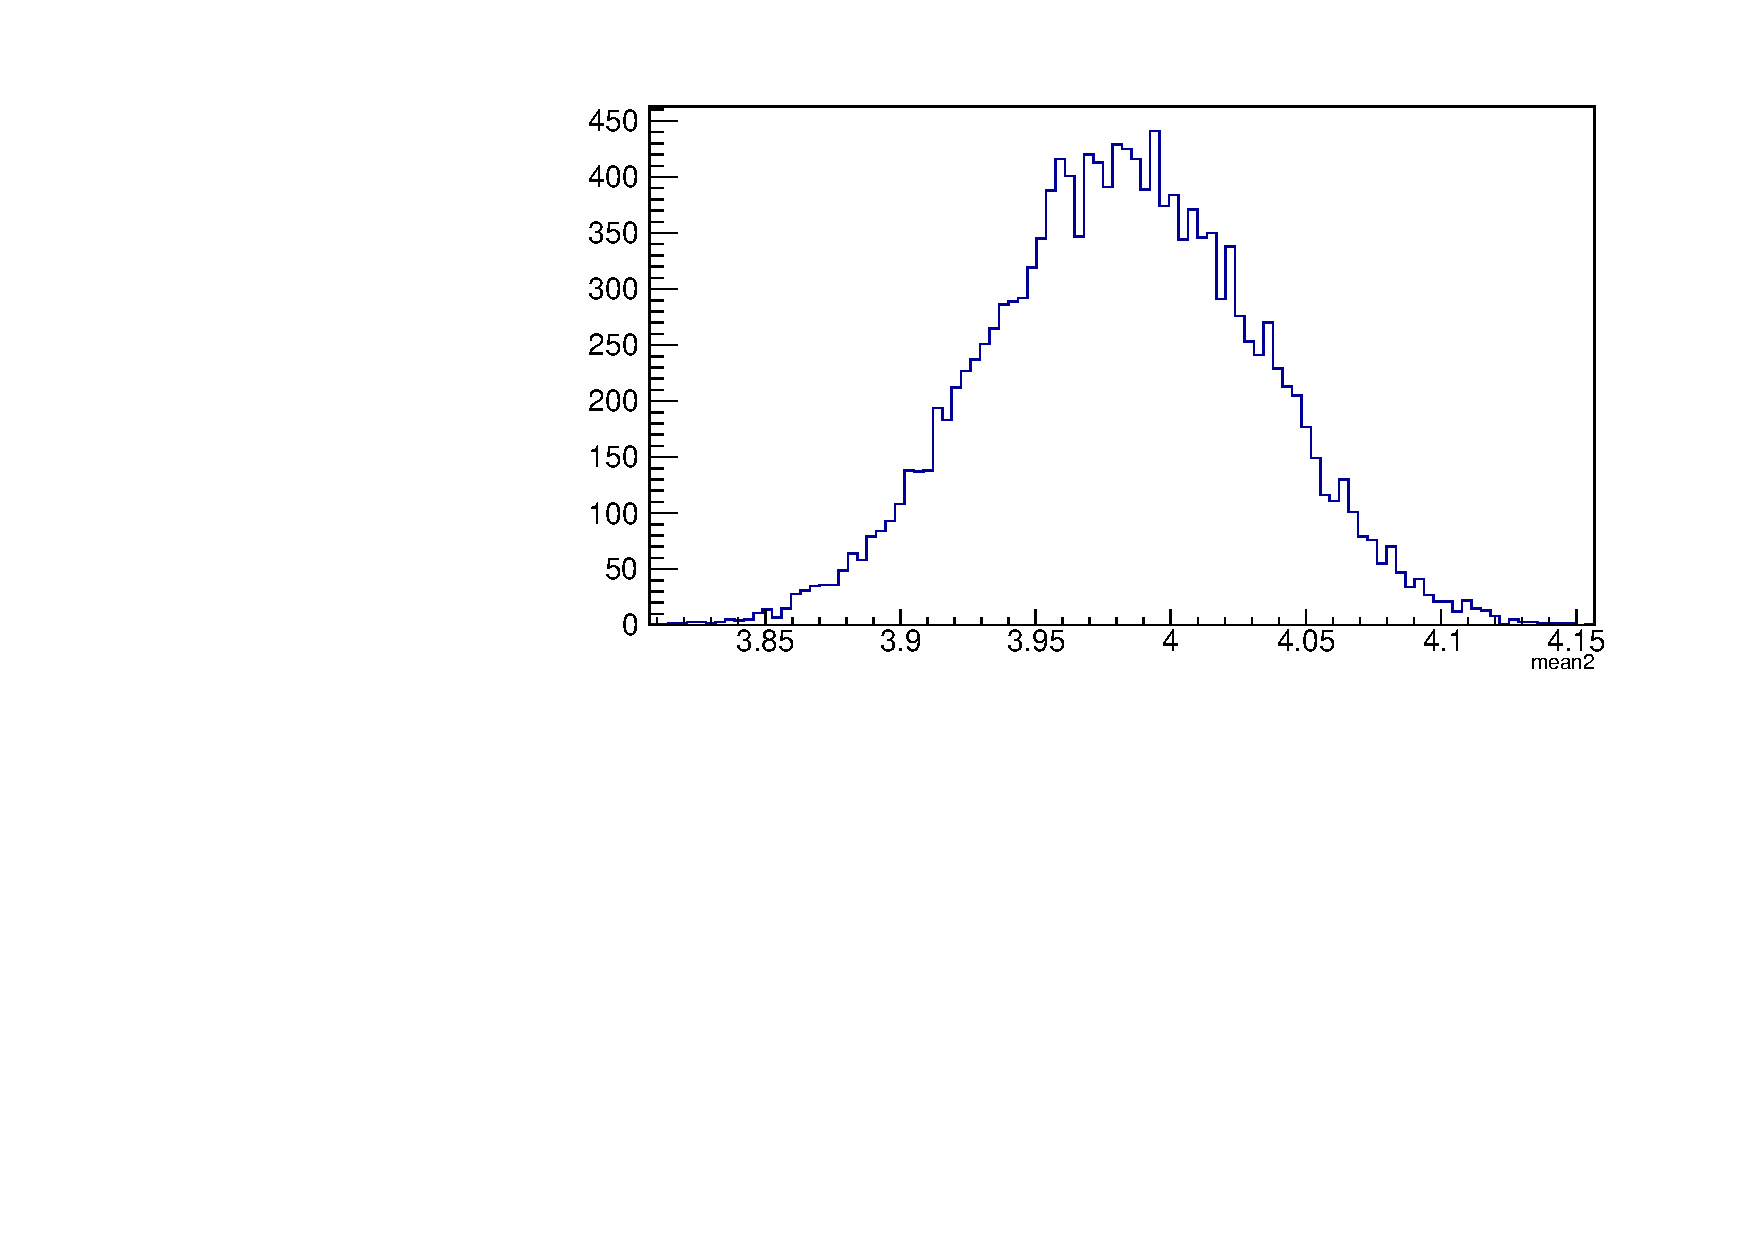
\includegraphics[width=0.8\textwidth]{RooMCMC/walkDisHis}
    \caption{Walk distribution of $\mu_2$ in equation \ref{eq:gausspdf} as a histogramm.}
    \label{fig:walkDisHis}
  \end{figure}
  This plot can be used to check, which error strategy should be used. If the walk distribution histogramm is gaussian, gaussian errors can be assumed. \\

  \item The scatterplot between two given parameters.
  \begin{figure}[H]
    \centering
    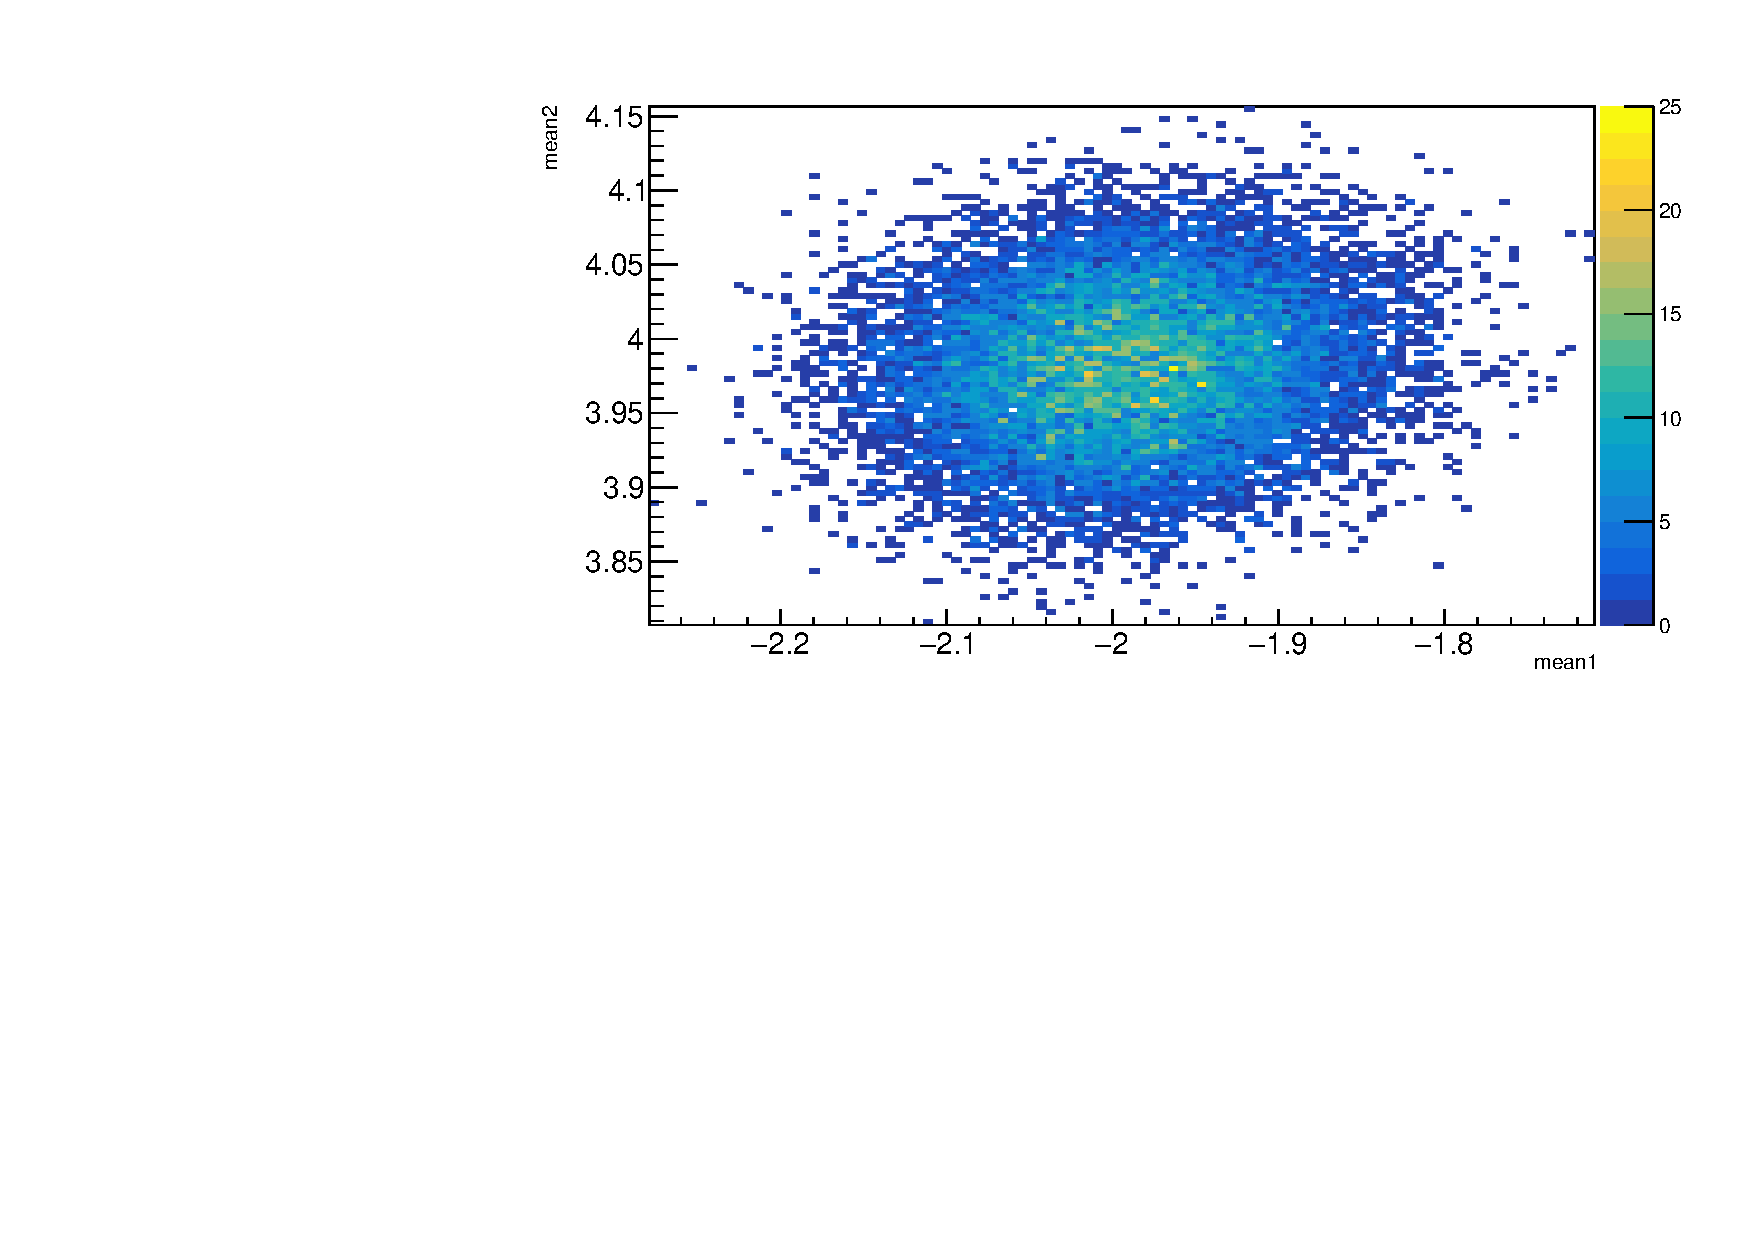
\includegraphics[width=0.8\textwidth]{RooMCMC/scatter}
    \caption{Scatterplot between $\mu_1$ and $\mu_2$ in equation \ref{eq:gausspdf}.}
    \label{fig:scatter}
  \end{figure}
  This plot shows the correlation between two parameters graphically.
\end{enumerate}











\begin{thebibliography}{100}
  \addcontentsline{toc}{section}{Bibliography}

  \bibitem{bib:lhc_img} CERN Accelerator Complex,
  \url{http://www.stfc.ac.uk/research/particle-physics-and-particle-astrophysics/large-hadron-collider/cern-accelerator-complex/}

  \bibitem{bib:lhcb_detector} Science and Technology Facilities Council article about LHCb ,
  \url{https://www.ppd.stfc.ac.uk/Pages/LHCb.aspx}

  \bibitem{bib:velo} VELO description,
  \url{http://lhcb-public.web.cern.ch/lhcb-public/en/Detector/VELO2-en.html}

  \bibitem{bib:rich} RICH description,
  \url{http://lhcb-public.web.cern.ch/lhcb-public/en/Detector/RICH2-en.html}

  \bibitem{bib:mag} Magnet description,
  \url{http://lhcb-public.web.cern.ch/lhcb-public/en/Detector/Magnet2-en.html}

  \bibitem{bib:trac} Tracker description,
  \url{http://lhcb-public.web.cern.ch/lhcb-public/en/Detector/Trackers2-en.html}

  \bibitem{bib:calo} Calorimeters description,
  \url{http://lhcb-public.web.cern.ch/lhcb-public/en/Detector/Calorimeters2-en.html}

  \bibitem{bib:muonSys} Muon system description,
  \url{http://lhcb-public.web.cern.ch/lhcb-public/en/Detector/Muon2-en.html}

  \bibitem{bib:sPlot} sPlot: a statistical tool to unfold data distributions,
  	arXiv:physics/0402083 [physics.data-an]

\end{thebibliography}

% \begin{appendix}
%   \section{ROC curves}
%   \label{app:roc}
%   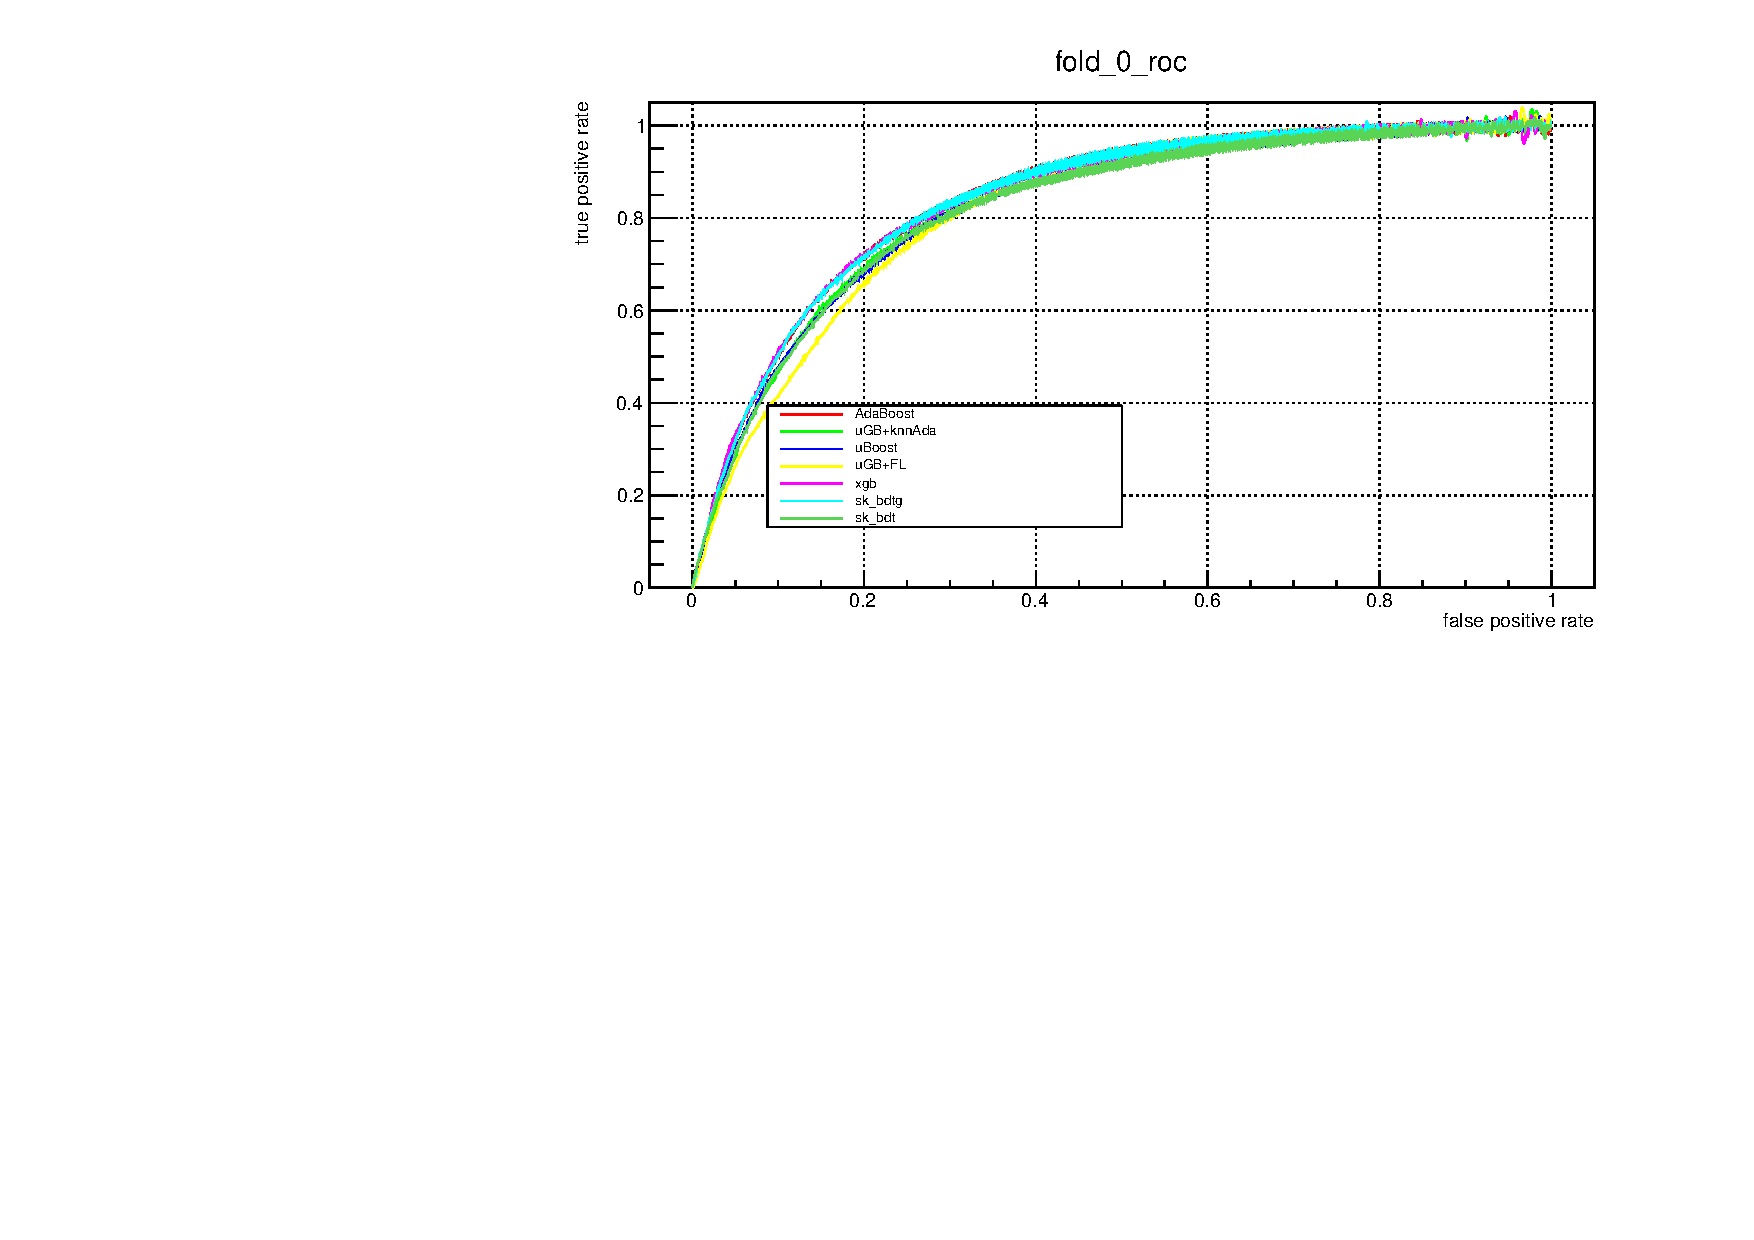
\includepdf[pages={-}]{roc.pdf}
%
%   \section{Learning Curves}
%   \label{app:lc}
%
%   \section{Correlation plots}
%   \label{app:corr}
%   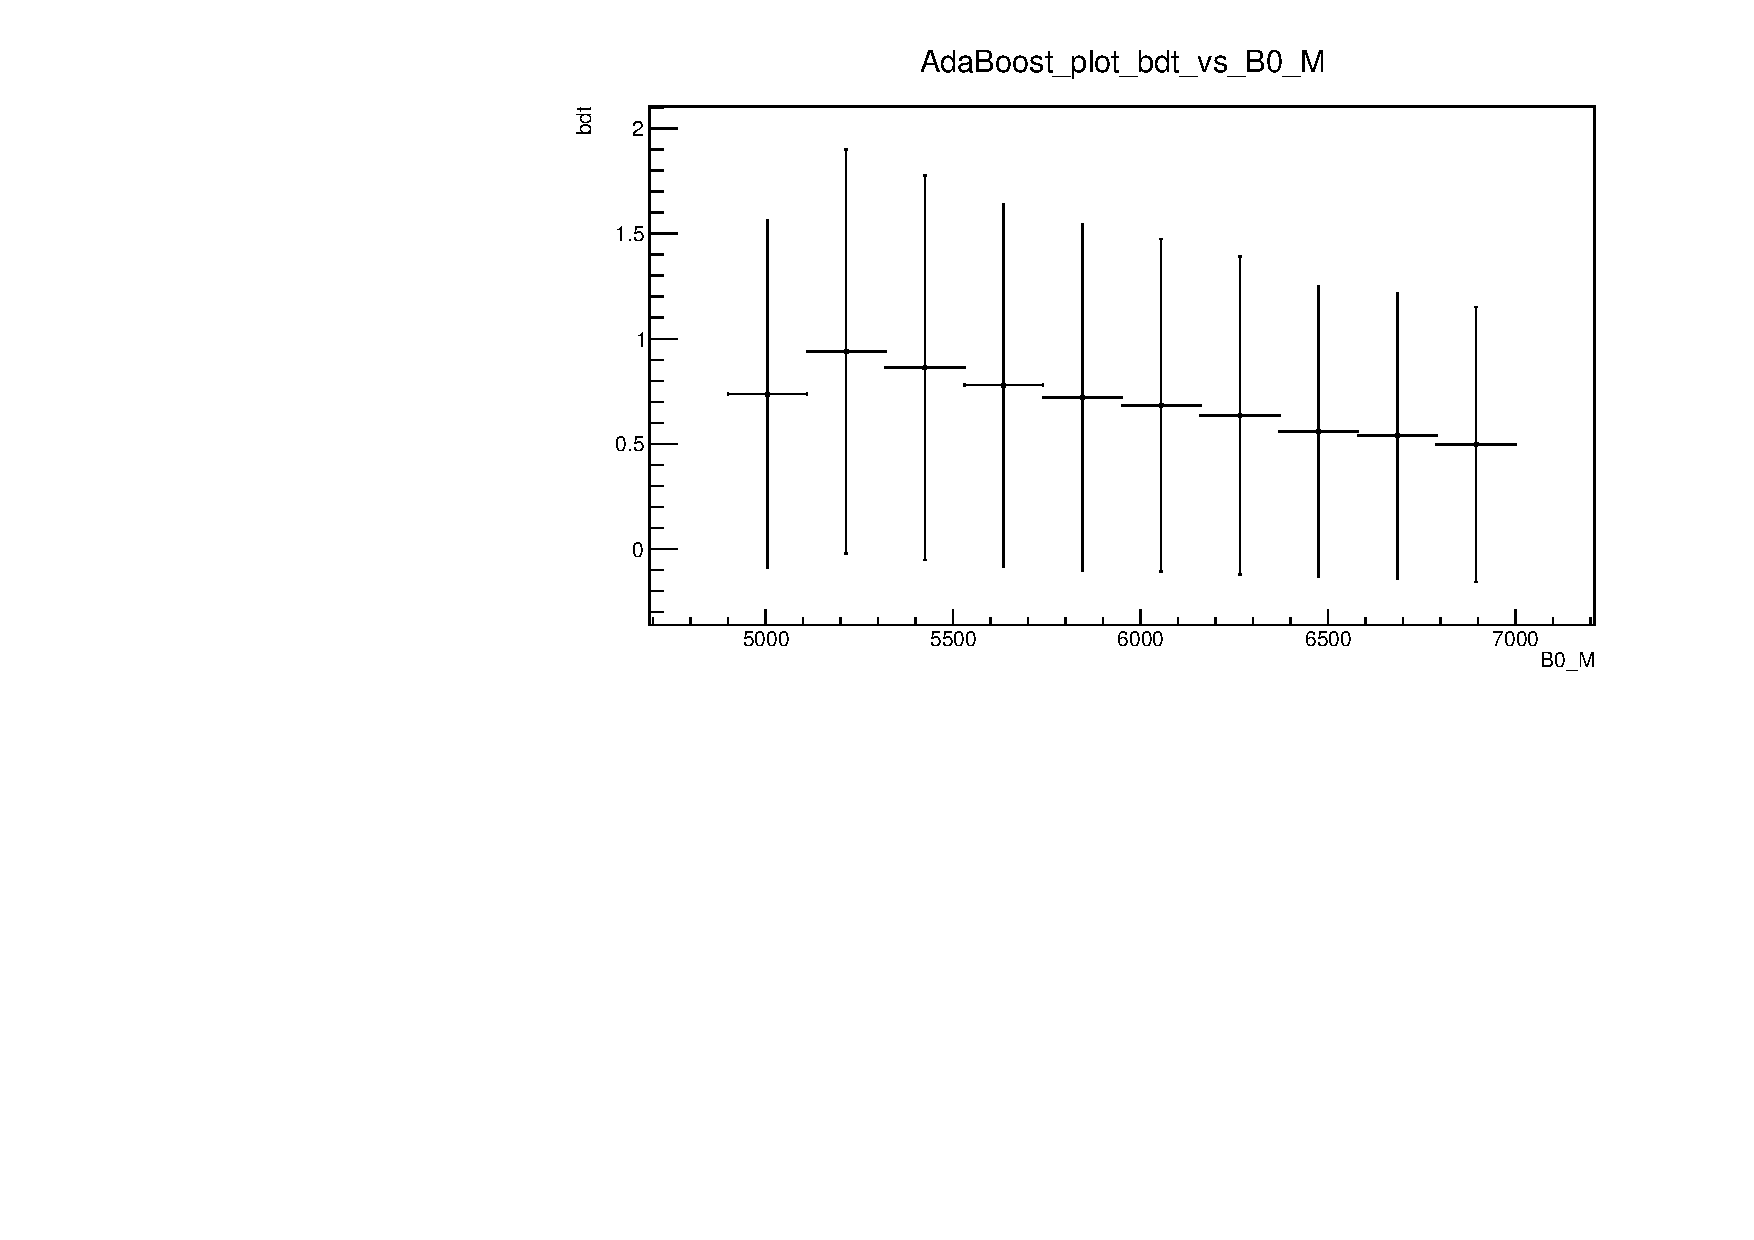
\includepdf[pages={-}]{Corplots.pdf}
%
%
% \end{appendix}

\end{document}
